\documentclass[12pt, a4paper, twoside, openright]{report}

\usepackage[T1]{fontenc}
\usepackage[spanish]{babel}
\usepackage{parskip}

\usepackage{hyperref}
\usepackage{graphicx}
\usepackage{float}
\makenoidxglossaries

\newglossaryentry{sacyl-conecta}
{
    name={sacyl conecta},
    description={Aplicación de acceso a la gestión de citas con su Centro de Salud, documentación clínica y más información}
}

\newglossaryentry{medora}
{
    name={medora},
    description={Sistema informático que gestiona la historia clínica, la receta electrónica y otros procesos clínicos de Atención Primaria en la sanidad castellano leonesa}
}

\newglossaryentry{tarjeta-sanitaria}
{
    name={tarjeta sanitaria},
    description={Programa informático con el que se gestiona la base de datos de tarjetas sanitarias de los usuarios de Castilla y León}
}

\newglossaryentry{incapacidad-temporal}
{
    name={incapacidad temporal},
    description={Situación en la que se encuentran los trabajadores impedidos temporalmente para trabajar debido a enfermedad común o profesional y accidente, sea o no de trabajo, mientras reciban asistencia sanitaria de la Seguridad Social}
}

\newglossaryentry{electrocardiograma}
{
    name={electrocardiograma},
    description={Procedimiento simple, indoloro y rápido que registra la actividad eléctrica de su corazón}
}

\newglossaryentry{guardia}
{
    name={guardia médica},
    description={Jornada laboral de 24 horas que realiza un facultativo en centros hospitalarios para garantizar la asistencia a los pacientes}
}

\newglossaryentry{matrona}
{
    name={matrona},
    description={Profesional sanitario que acompaña a la mujer en su embarazo, parto y posparto}
}

\newglossaryentry{ortopantomografías}
{
    name={ortopantomografías},
    description={Técnica de radiografía panorámica que se sirve de rayos X para ofrecer información detallada acerca de
    las estructuras dentales y la anatomía oral}
}

\newglossaryentry{volante}
{
    name={volante},
    description={Documento impreso que el profesional de la sanidad utiliza para prescribir pruebas diagnósticas, tratamientos, ingresos hospitalarios o intervenciones quirúrgicas}
}

\newglossaryentry{nodulos-tiroideos}
{
    name={nódulos tiroideos},
    description={Bultos sólidos o llenos de líquido que se forman dentro de la tiroides, una glándula pequeña ubicada en la base del cuello, justo encima del esternón}
}

\newglossaryentry{sintrom}
{
    name={sintrom},
    description={Medición de la determinación del INR (Razón Normalizada Internacional) o lo que es lo mismo, saber
    cuánto tarda una muestra de sangre en formar un coágulo}
}

\begin{document}

\title{Aplicación de técnicas de mejora continua en el centro de salud de Laguna de Duero}
\author{Luis Llamas Fernández}
\date{\today}
\maketitle

\thispagestyle{empty}

\chapter*{Resumen}
Este trabajo muestra un análisis de los distintos flujos de información y procesos que ocurren dentro de la sección 
administrativa del Centro de Salud de Laguna de Duero.
Para ello, se han hecho uso de técnicas de mejora continua y Lean 
Management, como la herramienta de los cinco porqués.
El estudio tiene como objetivo estandarizar las tareas que se realizan 
los distintos puestos además de descubrir las ineficiencias y, consecuentemente, plantear mejoras que ayuden a ofrecer un 
mejor servicio.
\keywords{sanidad, lean, bpmn, cinco porqués}

\setcounter{page}{1}

\chapter*{Abstract}
This work shows an analysis of the different information flows and processes that occur within the administrative section of the Laguna de Duero Health Centre.
For this purpose, we have made use of continuous improvement techniques and Lean  Management, such as the five whys tool.
The aim of the study is to standardise the tasks performed at the different workstations, as well as to discover inefficiencies and, consequently, to propose improvements that will help to offer a better service.
\keywords{healthcare, lean, bpmn, five whys}

\chapter*{Agradecimientos}
Quiero agradecer a todos los profesores que he tenido, tanto en la universidad como fuera de ella, por haber fomentado, aunque algunos más que otros, el desarrollo de mi curiosidad. También quiero agradecer a aquellos que me han formado como profesional y como persona, realizando un trabajo que nunca se podrá valorar lo suficiente. También a mi familia, que me ha dedicado todo su tiempo, todo su esfuerzo y todos sus recursos con tal de educarme y formarme lo mejor posible para afrontar la vida.

\tableofcontents

\chapter{Introducción}
\section{Contexto}

En los últimos años, tras el reciente periodo de pandemia y la situación económica del país, ha quedado patente la necesidad de una buena gestión sanitaria por parte de la administración con el fin de atender la creciente demanda de servicios asistenciales por parte de la población haciendo un uso eficiente de los recursos sanitarios.

La correcta gestión de los recursos en la sanidad es un tema que en menor o mayor grado concierne a todos los ciudadanos por un motivo principal: el derecho a la protección de la salud. Este se reconoce en el artículo 43 de la Constitución y se concreta en la Ley General de Sanidad (Ley 14/1986), que establece su financiación pública, universalidad y gratuidad; su descentralización autonómica y su integración en el Sistema Nacional de Salud (SNS). En definitiva, todas las personas tienen derecho a una atención sanitaria de calidad en condiciones de igualdad.

En base a esta premisa, recientemente se han sucedido numerosas manifestaciones en defensa de la sanidad pública por parte de distintas asociaciones y representantes que proponen un aumento de las partidas destinadas a equipos y personal del sistema sanitario público. Este trabajo va un paso más allá, presentando distinas propuestas en base a técnicas de mejora continua que mejoren la eficiencia de los recursos ya disponibles, tanto económicos como de personal.

Aunque durante los últimos años sí han habido numerosos proyectos de aplicación de técnicas de mejora continua en procesos sanitarios.

\section{Motivación personal}

El sector sanitario es un campo en el que no es común encontrar a un ingeniero industrial. Y cuando esto sucede, normalmente se suele asociar a aspectos técnicos como pueden ser el mantenimiento de las instalaciones térmicas y eléctricas o la ingeniería biomédica. Más extraño es, encontrar a un ingeniero involucrado en la mejora de procesos asistenciales.

Fue lo exótico de este campo junto con la posibilidad de poder dedicar mi tiempo a ayudar, aunque sea de forma indirecta, a los demás en un sector tan social como es el sanitario lo que me llevó a realizar este trabajo fin de máster.

La ingeniería de procesos, al menos tal y como se imparte en la carrera, está orientada principalmente a la industria manufacturera en cuanto a producción de bienes de equipo. Todas las metodologías aprendidas, kaizen, 5s, JIT o kanban son muchas veces aplicables a los procesos asistenciales sustituyendo el producto material por personas.

\section{Objetivos}

El objetivo principal de este trabajo fin de máster es analizar la problemática y plantear propuestas de mejora en el centro de salud de Laguna de Duero.

Para conseguir este objetivo se plantean los siguientes subobjetivos.
\begin{enumerate}
    \item Crear un grupo de trabajo con los representantes del personal administrativo del centro.
    \item Realizar una lista de tareas comunes al personal administrativo tanto de ventanilla como de interior
    \item Elaborar una tabla con los problemas de mayor importancia y sus respectivas causas
    \item Plantear mejoras en los distintos procesos que se llevan a cabo
\end{enumerate}

\section{Alcance}

El área de estudio comprende la sección administrativa del centro de salud de Laguna de Duero (Valladolid) perteneciente al Área de Salud Valladolid Oeste. La decisión de elegir este centro fue motivada por la gran variedad de servicios que ofrece: extracciones, salud bucodental, fisioterapia, radioogía y un punto de atención continuada. Además, el centro se encuentra a medio camino entre la tipología rural y urbana haciendolo idóneo para realizar este proyecto en vista de aplicarlo al resto de centros de salud del área.

Para llevar a cabo el estudio se han hecho uso de distintas técnicas de mejora continua de procesos:
\begin{itemize}
    \item Ciclo PDCA: Plan-Do-Check-Act
    \item Cuadro de los cinco porqués
    \item Gemba walks
    \item Análisis de las tres M's: muri, mura y muda
    \item Mapa VSM: Value Stream Mapping
\end{itemize}

Dado que este proyecto se ha propuesto desde la Dirección de Gestión de la Gerencia de Atención Primaria, solamente se ha involucrado al personal administrativo. Si se cumplen los objetivos, en el futuro se pretende incluir en el grupo de trabajo a representantes de los demás grupos de interés involucrados en los procesos del centro de salud: médicos, enfermeras, auxiliares de enfermería y celadores entre otros.

\section{Estructura memoria}

Esta memoria sigue la estructura especificada en la guía docente para la asignatura TFM del Máster en Ingeniería Industrial de la Escuela de Ingenieros Industriales (Universidad de Valladolid).

Siguiendo al presente capítulo de introducción, donde se expone el contexto, la motivación, el alcance y los objetivos de este trabajo, se encuentran los siguientes capítulos:

\begin{itemize}
    \item Capítulo 2. Atención Primaria en el Área de Salud Valladolid Oeste
    \item Capítulo 3. Herramientas de mejora continua en el sector sanitario
    \item Capítulo 4. Desarrollo
    \item Capítulo 5. Estudio económico
    \item Capítulo 6. Conclusiones
\end{itemize}

Finalmente se adjunta las referencias bibliográficas utilizadas.


\chapter{Centro de Salud de Laguna de Duero}
En el siguiente capítulo se desarrolla la estructura organizativa y el funcionamiento de la Atención Primaria dentro del Área de Salud Valladolid Oeste así como la situación del Centro de Salud de Laguna de Duero dentro de la organización.

\section{Área de Salud Valladolid Oeste}

El Área de Salud Valladolid Oeste (ASVAO) presta asistencia sanitaria a la población de aproximadamente la mitad de la provincia de Valladolid, la situada geográficamente en la zona oeste.
Esta atención sanitaria se provee en sus dos niveles asistenciales: Atención Primaria (con 17 Zonas Básicas de Salud) y Atención Especializada (con el Hospital Universitario Rio Hortega y el Centro de Especialidades de Arturo Eyries).
Esta organización es fruto del trabajo integrado de las Gerencias de Atención Primaria y Especializada.

El Área de Salud Valladolid Oeste (ASVAO) forma parte del Sistema Público de Salud de Castilla y León, el cual comprende el conjunto de actuaciones y recursos públicos de la Administración Sanitaria de la Comunidad Autónoma y de las Corporaciones Locales, cuya finalidad es la promoción y protección de la salud en todos sus ámbitos, la prevención de la enfermedad, la asistencia sanitaria y la rehabilitación, todo ello bajo una perspectiva de asistencia sanitaria integral \cite{noauthor_ley_2010}.

El Hospital Universitario Río Hortega fue inaugurado como centro hospitalario el 24 de Julio de 1953.
En ese momento disponía de 310 camas y 72 cunas.
Tras más de 50 años ubicado en pleno centro (cerca de la plaza de San Pablo), se trasladó a un nuevo edificio en el año 2008, esta vez situado a las afueras de la ciudad, en el barrio de las Delicias.
En estos momentos cuenta con 640 camas instaladas y se configura como un hospital general, universitario y de tercer nivel.
Además de prestar atención sanitaria al Área de Salud Valladolid Oeste, para determinadas prestaciones actúa como “Servicio de Referencia”, ampliando su cobertura a toda la provincia de Valladolid o incluso a varias provincias limítrofes.
En algunos casos presta servicio a toda la Comunidad Autónoma.

Según ACUERDO 111/2008 de 23 de octubre de la Junta de Castilla y León \cite{noauthor_bocyl_2008}, se reestructura el Área de Salud de Valladolid Oeste y el Área de Salud de Valladolid Este.

La apertura del nuevo Hospital Universitario Río Hortega, que cambia de ubicación, hace necesaria la adaptación del mapa sanitario del Área de Salud de Valladolid Oeste, pasando las Z.B.S. Centro Gamazo, Z.B.S. la Victoria, Z.B.S. Rural I, Z.B.S. Cigales a pertenecer al Área Este de Valladolid y las Z.B.S. Delicias I y Z.B .S. Delicias II pasan a pertenecer al Área Oeste de Valladolid.

Al frente de la organización se han sucedido los siguientes nombramientos en los últimos años: Por Orden SAN/465/2012 de 18 de junio \cite{noauthor_orden_2012} se nombró Gerente de Atención Especializada a D. Alfonso Montero Moreno, posteriormente por resolución de 15 de febrero de 2012 del Gerente Regional de Salud se acumularon las funciones de Gerente de Atención Primaria a las de Gerente de Atención Especializada.
El 18 de julio de 2015 fue nombrado como Gerente de Atención Primaria D. Eduardo García Prieto.
Por último en el año 2018 a través de Orden SAN/901/2018 de 10 de agosto \cite{noauthor_orden_2018} se nombró Gerente de Atención Especializada a D. José Miguel García Vela.

A partir del mes de marzo de 2017 todo el personal de la Gerencia de Atención Primaria se integró a trabajar en las instalaciones del HURH junto a de los diferentes servicios correspondientes.

\section{Atención Primaria}

\subsection{Cartera de servicios}

El Área de Salud Valladolid Oeste (ASVAO) es la organización a la que se adscribe todo el dispositivo sanitario del Área, compuesto por los 17 Centros de A. Primaria y por el Hospital Universitario Río Hortega.
El objetivo primordial de esta organización es la prestación de asistencia sanitaria a la población del Área Oeste de Valladolid, tanto en Atención Primaria, en Atención Especializada como en Atención Sociosanitaria (esta última compartida con la Gerencia Regional de Servicios Sociales).

La Atención Primaria es el nivel básico e inicial de atención, que garantiza la globalidad y continuidad de ésta a lo largo de la vida del paciente, actuando como gestor y coordinador de casos y regulador de flujos.
Comprende actividades de promoción de la salud, educación sanitaria, prevención de la enfermedad, asistencia sanitaria, mantenimiento y recuperación de la salud, así como la rehabilitación física y el trabajo social.

La Atención Especializada comprende las actividades asistenciales, diagnósticas, terapéuticas y de rehabilitación y cuidados, así como aquellas de promoción de la salud, educación sanitaria y prevención de la enfermedad, cuya naturaleza aconseja que se realicen en ese nivel.
La Atención Especializada garantizará la continuidad de la atención integral al paciente, una vez superadas las posibilidades de la Atención Primaria y hasta que aquel pueda reintegrarse en dicho nivel.
Prestará además, servicios de hospitalización en régimen de internamiento, asistencia especializada en consultas, hospital de día (médico y quirúrgico), atención paliativa a enfermos terminales, salud mental y rehabilitación en pacientes con déficit funcional recuperable.

La Atención Sociosanitaria comprende el conjunto de cuidados destinados a aquellos enfermos, generalmente crónicos, que por sus especiales características pueden beneficiarse de la actuación simultánea y sinérgica de los servicios sanitarios y sociales para aumentar su autonomía, paliar sus limitaciones o sufrimientos y facilitar su reinserción social.
En el ámbito sanitario, la Atención Sociosanitaria comprenderá los cuidados sanitarios de larga duración, la atención sanitaria a la convalecencia y la rehabilitación en pacientes con déficit funcional recuperable.

La cartera de servicios en Atención Primaria de Valladolid Oeste, Tabla~\ref{tab:cartera-servicios}, está compuesta por:

\begin{table}
    \centering
    \begin{tabular}{l}
        \toprule
        Servicios                                             \\
        \midrule
        Medicina familiar y comunitaria                       \\
        Pediatría                                             \\
        Enfermería                                            \\
        Unidad de salud bucodental                            \\
        Unidad de atención a la mujer                         \\
        Fisioterapia                                          \\
        Extracciones laboratorio                              \\
        Radiología                                            \\
        Urgencias                                             \\
        Asistemcia social                                     \\
        Cirugía menor                                         \\
        Diagnóstico ecográfico                                \\
        Farmacia                                              \\
        Unidad administrativa de citas y atención al paciente \\
        Prevención y promoción de la salud                    \\
        \bottomrule
    \end{tabular}
    \caption{Cartera de servicios en atención primaria}
    \label{tab:cartera-servicios}
\end{table}

Existe un amplio capítulo de actuaciones dirigidas a la Prevención y Promoción de la Salud, en el que se incluyen, entre otros, programas de vacunación infantil, programas de vacunación en el adulto, desarrollo de actividades preventivas en el adulto sano, prevención de obesidad infantil, atención a pacientes crónicos (hipertensión arterial, dislipemias, diabetes, EPOC, etc.), atención al paciente crónico pluripatológico complejo, prevención precoz de cáncer de mama, de colon, deshabituación tabáquica, atención a pacientes ancianos de riesgo o en situación terminal, violencia de género, etc.

\subsection{Mercado servido}

El Área de Salud Valladolid Oeste da cobertura asistencial principalmente a su área de referencia.
También es referente en algunos servicios sanitarios para las Áreas de Salud de Valladolid Este, Segovia, Palencia, Burgos y Soria.

Dentro de la Atención Primaria tenemos las Zonas Básicas de Salud mostradas en la Tabla \ref{tab:zonas-basicas}.

\begin{table}
    \centering
    \begin{tabular}{cll}
        \toprule
        \multicolumn{2}{c}{Zonas   Básicas de Salud} & Centro de Salud                                      \\
        \midrule
        \multirow{8}{*}{Urbanas}                     & ZBS Arturo Eyries       & CS Arturo Eyries           \\
                                                     & ZBS Campo Grande        & CS Campo Grande            \\
                                                     & ZBS Esperanto           & CS Plaza del Ejército      \\
                                                     & ZBS Huerta del Rey      & CS Huerta del Rey          \\
                                                     & ZBS Parquuesol          & CS Parquesol               \\
                                                     & ZBS Valladolid Sur      & CS Parque Alameda-Covaresa \\
                                                     & ZBS Delicias I          & CS Delicias I              \\
                                                     & ZBS Delicias II         & CS Delicias II             \\
        \midrule
        \multirow{11}{*}{Rurales}                    & ZBS Laguna de Duero     & CS Laguna de Duero         \\
                                                     & ZBS Tordesillas         & CS Tordesillas             \\
                                                     & ZBS Mayorga             & CS Mayorga                 \\
                                                     & ZBS Medina de Rioseco   & CS Medina de Rioseco       \\
                                                     & ZBS Mayorga             & CS Mayorga                 \\
                                                     & ZBS Medina de Rioseco   & CS Medina de Rioseco       \\
                                                     & ZBS Mota del Marqués    & CS Mota del Marqués        \\
                                                     & ZBS Pisuerga            & CS Pisuerga                \\
                                                     & ZBS Valladolid Rural II & CS Zaratán                 \\
                                                     & ZBS Villafrechós        & CS Villafrechós            \\
                                                     & ZBS Villalón            & CS Villalón                \\
        \bottomrule
    \end{tabular}
    \caption{Relación de Zonas Básicas de Salud y Centros de Salud}
    \label{tab:zonas-basicas}
\end{table}

\subsection{Tamaño de la organización}

El Área de Salud Valladolid Oeste dispone de dos centros de gasto diferenciados y el 100\% de sus recursos provienen de la Consejería de Sanidad de Castilla y León. En las tablas \ref{tab:gastos-primaria} se muestran los presupuestos anuales del Área de Salud Valladolid Oeste.

\begin{table}
    \centering
    \begin{tabular}{lrrr}
        \toprule
        Año                              & 2016              & 2017              & 2018              \\
        \midrule
        Inversiones                      & 260317            & 353879            & 293654            \\
        Compras a proveedores            & 2054867           & 2141010           & 2157458           \\
        \textbf{TOTAL COMPRAS}           & \textbf{2315184}  & \textbf{2494889}  & \textbf{2451112}  \\
        \midrule
        Productos farmacéuticos          & 1349              & 1488              & 1488              \\
        Material sanitario               & 894527            & 980114            & 943458            \\
        Gastos externos                  & 1395160           & 1423618           & 1354330           \\
        Otros gastos de explotación      & 1158991           & 1159408           & 1212512           \\

        \textbf{TOTAL G. FUNCIONAMIENTO} & \textbf{3450027}  & \textbf{3564628}  & \textbf{3511788}  \\
        \midrule
        Gastos de personal               & 39835467          & 41112893          & 42048766          \\
        \textbf{TOTAL G. EXPLOTACIÓN}    & \textbf{43285494} & \textbf{44677521} & \textbf{45560554} \\
        \bottomrule
    \end{tabular}
    \caption{Distribución de gastos de Atención Primaria en euros}
    \label{tab:gastos-primaria}
\end{table}

\section{Centro de Salud de Laguna de Duero}

El Centro de Salud de Laguna de Duero se encuentra localizado en la avenida Madrid, Nº6 dentro del municipio con el mismo nombre de la provincia de Valladolid. En la Figura \ref{fig:localizacion-centro} se muestra la ubicación a distintos niveles geográficos.

\begin{figure}[H]
    \centering
    \begin{subfigure}[H]{0.48\textwidth}
        \centering
        \includegraphics*[width=\textwidth]{img/mapa-comunidad.png}
        \caption{Comunidad autónoma de Castilla y León}
    \end{subfigure}
    \hfill
    \begin{subfigure}[H]{0.48\textwidth}
        \centering
        \includegraphics*[width=\textwidth]{img/mapa-provincia.png}
        \caption{Provincia de Valladolid}
    \end{subfigure}
    \hfill
    \begin{subfigure}[H]{0.48\textwidth}
        \centering
        \includegraphics*[width=\textwidth]{img/mapa-municipio.png}
        \caption{Municipio de Laguna de Duero}
    \end{subfigure}
    \hfill
    \begin{subfigure}[H]{0.48\textwidth}
        \centering
        \includegraphics*[width=\textwidth]{img/centro-salud.jpg}
        \caption{Centro de Salud}
    \end{subfigure}
    \caption{Localización geográfica del Centro de Salud de Laguna de Duero}
    \label{fig:localizacion-centro}
\end{figure}

\subsection{Información demográfica}

Comparado con otros centros, el de Laguna de Duero se caracteriza por tener el mayor número de población asignada junto con el centro de Parquesol. Además, respecto a otros centros de tipo rural la población es relativamente joven como se puede observar en la Tabla \ref{tab:poblacion}.

\begin{table}[H]
    \centering
    \begin{tabular}{lrrrrrrr}
        \toprule
        ZBS                      & 0-14          & \%               & 14-64          & \%               & 64-$\infty$   & \%               & Total          \\
        \midrule
        Arturo Eyries            & 1994          & 10.6\%           & 11760          & 62.5\%           & 5055          & 26.9\%           & 18809          \\
        Campo Grande             & 1426          & 9.6\%            & 9360           & 63.1\%           & 4054          & 27.3\%           & 14840          \\
        Delicias I               & 3371          & 12.9\%           & 17753          & 67.8\%           & 5047          & 19.3\%           & 26171          \\
        Delicias II              & 2583          & 13.9\%           & 11916          & 64.0\%           & 4118          & 22.1\%           & 18617          \\
        Esperanto                & 1653          & 8.8\%            & 11700          & 62.2\%           & 5446          & 29.0\%           & 18799          \\
        Huerta del Rey           & 3258          & 12.9\%           & 16194          & 64.1\%           & 5813          & 23.0\%           & 25265          \\
        \textbf{Laguna de Duero} & \textbf{3855} & \textbf{13.53\%} & \textbf{19937} & \textbf{69.98\%} & \textbf{4696} & \textbf{16.48\%} & \textbf{28488} \\
        Mayorga                  & 144           & 5.4\%            & 1538           & 57.5\%           & 994           & 37.1\%           & 2676           \\
        Medina de Rioseco        & 636           & 9.8\%            & 4209           & 65.1\%           & 1616          & 25.0\%           & 6461           \\
        Mota del Marqués         & 85            & 4.5\%            & 1059           & 56.5\%           & 732           & 39.0\%           & 1876           \\
        Parquesol                & 3269          & 11.4\%           & 20635          & 72.2\%           & 46751         & 16.4\%           & 28579          \\
        Pisuerga                 & 4490          & 19.3\%           & 16524          & 71.0\%           & 2251          & 9.7\%            & 23265          \\
        Tordesillas              & 1160          & 10.1\%           & 7552           & 66.0\%           & 2741          & 23.9\%           & 11453          \\
        Valladolid Rural II      & 1611          & 18.4\%           & 5979           & 68.1\%           & 1184          & 13.5\%           & 8774           \\
        Valladolid Sur           & 3050          & 13.7\%           & 15714          & 70.6\%           & 3493          & 15.7\%           & 22257          \\
        Villafrechós             & 142           & 6.6\%            & 1302           & 60.9\%           & 695           & 32.5\%           & 2139           \\
        Villalón de Campos       & 146           & 6.4\%            & 1347           & 58.7\%           & 801           & 34.9\%           & 2294           \\
        \midrule
        TOTAL ASVAO              & 32873         & 12.6\%           & 174479         & 66.9\%           & 53411         & 20.5\%           & 260763         \\
        \bottomrule
    \end{tabular}
    \caption{Población por tramos quinquenales y sexo en el año 2020}
    \label{tab:poblacion}
\end{table}

\chapter{Metodología lean en sanidad}
En el siguiente capítulo se desarollan las herramientas de gestión lean utilizadas en el proyecto además de exponer una breve explicación de la metodología y su implantación en los últimos años.

\section{Definición de la metodología lean}

La gestión Lean es un concepto moderno para la optimización de procesos en toda la cadena de valor \cite{helmold_progress_2019}.
Se centra en hacer que las ineficiencias, o desperdicios, sean transparentes y en alterarlas para convertirlas en actividades que añadan valor \cite{helmold_global_2016}.
La cadena de valor abarca en este contexto desde los proveedores, pasando por las propias operaciones, hasta los clientes \cite{slack_operations_2010}.
Las ineficiencias son todo aquello, por ejemplo, una actividad, un proceso y un producto, que se considera algo por lo que los clientes no están dispuestos a pagar o a gastar medios financieros.

El cliente es el punto central del concepto lean.
Los principales objetivos de la filosofía lean son crear valor para el cliente mediante la optimización de los recursos y crear un flujo de trabajo constante basado en las demandas reales de los clientes \cite{ohno_toyota_1988}. Busca eliminar cualquier pérdida de tiempo, esfuerzo o dinero identificando cada paso en un proceso de negocio y luego revisando o recortando los pasos que no crean valor \cite{bertagnolli_lean_2018}.

La filosofía tiene sus raíces en Japón pero actualmente está ampliamente extendida por todo el mundo.
La gestión lean facilita el liderazgo y la responsabilidad compartida mientras que la mejora continua garantiza que cada empleado contribuya al proceso de mejora.
La metodología actúa como guía para construir una organización sólida y de éxito que progresa constantemente, identificando los problemas reales y resolviéndolos.
Lean se basa en el sistema de producción Toyota, creado a finales de los años cincuenta.
Toyota puso en práctica los cinco principios de la gestión ajustada con el objetivo de reducir la cantidad de procesos que no producían valor, lo que se conoce como \textit{Toyota Way}.

Al aplicar los cinco principios, se encontraton mejoras significativas en eficiencia, productividad, rentabilidad y duración de los ciclos.
Lean incorpora cinco principios rectores que son utilizados por los directivos de una organización como directrices de la metodología \cite{helmold_progress_2019}. Los cinco principios son:

\begin{itemize}
    \item Identificar el valor en todos los procesos de la cadena de valor.
    \item Realización de mapas de flujo de valor.
    \item Crear un flujo de trabajo continuo.
    \item Establecer un sistema \textit{pull} en el que los clientes sean el centro de atención.
    \item Facilitar una cultura de mejora continua.
\end{itemize}

Identificar el valor, el primer paso en la gestión lean, significa encontrar el problema que el cliente necesita resolver y convertir el producto en la solución.
En concreto, el producto debe ser la parte de la solución por la que el cliente esté dispuesto a pagar.
Cualquier proceso o actividad que no añada valor, es decir, que no aporte utilidad y el cliente no está dispuesto a pagar por ello, importancia o valor al producto fnal se considera residuo y debe eliminarse \cite{liker_toyota_2006}.

El mapeo del flujo de trabajo de la empresa, incluyendo todas las acciones y personas que contribuyen al proceso de creación y entrega del producto final al consumidor, se realiza con la herramienta de VSM\footnote{Las siglas corresponden con el término Value Stream Mapping}.
Trazar la cadena de valor ayuda a los directivos a visualizar qué procesos están dirigidos por qué equipos y a identificar a las personas responsables de medir, evaluar y mejorar el proceso.
La visualización ayuda a los directivos a determinar qué partes del sistema no aportan valor al flujo de trabajo \cite{slack_operations_2010}.

Crear un flujo de valor continuo significa garantizar que el flujo de trabajo de cada equipo progrese sin problemas y evitar las interrupciones o cuellos de botella que pueden producirse con el trabajo en equipos interfuncionales.
\textit{Kanban}, una técnica de gestión ajustada que utiliza una señal visual para desencadenar la acción, se utiliza para facilitar la comunicación entre equipos para que puedan abordar lo que hay que hacer y cuándo hay que hacerlo.

Desarrollar un sistema \textit{pull} asegura que el flujo de trabajo continuo se mantenga estable y garantiza que los equipos entreguen las asignaciones de trabajo más rápido y con menos esfuerzo. Un sistema pull es una técnica lean específica que reduce los residuos de cualquier producción. Garantiza que sólo se inicie un nuevo trabajo si hay demanda del mismo, lo que ofrece la ventaja de minimizar los gastos generales y optimizar los costes de almacenamiento.

El último principio es la mejora continua y puede considerarse el paso más importante del método de gestión ajustada.
Facilitar la mejora continua se refiere a una serie de técnicas que se utilizan para identificar lo que una organización ha hecho, lo que necesita hacer, los posibles obstáculos que puedan surgir y cómo todos los miembros de la organización pueden mejorar sus procesos de trabajo.
El sistema lean no está aislado ni es inmutable, por lo que pueden surgir problemas en cualquiera de los otros cuatro pasos.
Asegurarse de que todos los empleados contribuyen a la mejora continua del flujo de trabajo protege a la organización cuando surgen problemas.
La dirección debe crear un entorno y una cultura en los que todos los empleados puedan trabajar de acuerdo con los cinco principios \cite{ohno_toyota_1988,bertagnolli_lean_2018}.

\section{La gestión lean en el sector sanitario}

Lean parte del rechazo al despilfarro. Atribuido a Taiichi Ohno, el sistema Lean se desarrolló en los años 50 y 60 para ofrecer la mejor calidad, el menor coste y el menor plazo de entrega mediante la eliminación de los residuos.
El término japonés para lo que las empresas estadounidenses suelen clasificar como despilfarro es \textit{muda} y fue definido por Fujio Cho de Toyota como "cualquier cosa que no sea la cantidad mínima de equipo, espacio y tiempo del trabajador, que son absolutamente esenciales para añadir valor al producto" \cite{helmold_lean_2020}.

La presencia de este tipo de residuos en un sistema repercute negativamente en el plazo de entrega, el coste y la calidad.
A principios de los años 80, empresas de otros sectores, como el sanitario, comprendieron que la introducción de los principios lean conllevaría varias ventajas.
El despilfarro en la sanidad puede describirse, entre otros elementos, en el transporte excesivo de medicamentos o pacientes, el tiempo de espera para los tratamientos o la infrautilización de equipos y máquinas en los hospitales. Además, las duplicaciones e ineficiencias del personal de enfermería también pueden repercutir en la creación de residuos.

Aunque la metodología de mejora empresarial lean se desarrolló inicialmente para mejorar la calidad y la productividad de las fábricas de automóviles, se ha utilizado con gran éxito en industrias y entornos de todo tipo, como el desarrollo de software, la administración pública, el comercio minorista y otros entornos de servicios.
Las organizaciones sanitarias, en particular, han descubierto que el enfoque puede utilizarse para reducir costes y mejorar la calidad y la satisfacción de los pacientes al mismo tiempo \cite{millard_how_nodate}.
Uno de los principios básicos del lean es la eliminación del despilfarro, que se define como todo aquello que no añade valor al cliente.
Los profesionales se centran en ocho tipos específicos de residuos.
Son tan comunes en la sanidad como en la industria.
Por lo tanto, la gestión ajustada tiene como objetivo eliminar, por ejemplo, los tiempos de espera o el exceso de medicación como se muestra en la Tabla~\ref{tab:timwood}.

\begin{table}
    \centering
    \begin{tabular}{llp{10cm}}
        \toprule
        Letra & Despilfarro     & Definición                                                                         \\
        \midrule
        T     & Transport       & Movimiento excesivo de personas, información o materiales                          \\
        I     & Inventory       & Stock excesivo y retraso en la información o productos                             \\
        M     & Motion          & Cualquier movimiento que no añada valor al producto o al proceso                   \\
        W     & Waiting         & Largos periodos de inactividad de personas, información, maquinaria o   materiales \\
        O     & Overutilization & Producir más o antes de que lo requiera el cliente                                 \\
        O     & Overprocessing  & Utilización de las herramientas, procedimientos o sistemas incorrectos             \\
        D     & Defects         & Errores frecuentes en los trámites o en la calidad del producto                    \\
        \bottomrule
    \end{tabular}
    \caption{TIMWOOD, el acrónimo que define los siete despilfarros en la industria}
    \label{tab:timwood}
\end{table}

\subsection{Transporte}

El despilfarro del transporte se produce cuando los materiales se trasladan de un lugar a otro de forma ineficaz. En sanidad se produce cuando:

\begin{itemize}
    \item Los pacientes son trasladados de un departamento a otro o de una habitación a otra
    \item Los medicamentos se trasladan de la farmacia al lugar donde se necesitan
    \item Los suministros se trasladan del almacén a la planta
\end{itemize}

Algunos de estos transportes se consideran residuos "necesarios" que hay que minimizar aunque no puedan eliminarse por completo.

\subsection{Inventario}

Los fabricantes han adoptado en gran medida un enfoque de inventario justo a tiempo para reducir los costes relacionados con el almacenamiento, el movimiento, el deterioro y el desperdicio.
Las organizaciones sanitarias buscan hacer lo mismo en lo que se refiere a:

\begin{itemize}
    \item Medicación que esté cerca de la fecha de caducidad
    \item Exceso de consumibles
    \item Formularios preimpresos
    \item Exceso de material de cabecera
\end{itemize}

\subsection{Movimiento}

El movimiento se refiere al desplazamiento innecesario de personas dentro de una instalación.
Este ocurre cuando:

\begin{itemize}
    \item La distribución de las oficinas o del hospital no es coherente con el flujo de trabajo.
    \item Los suministros no se almacenan donde se necesitan
    \item Los equipos no están bien situados
\end{itemize}

El primer paso para combatir los despilfarros del lean es reconocerlos dentro de su organización.
En la mayoría de los casos, el examen de cada uno de estos factores específicos que contribuyen con frecuencia al despilfarro conduce al descubrimiento de múltiples oportunidades de mejora.
También podemos esforzarnos por eliminar el despilfarro (incluidos los clics del ordenador) en los sistemas de software.

\subsection{Esperas}

En la fabricación, la espera se produce cuando las piezas no pueden salir o cuando los miembros del equipo no pueden realizar sus tareas debido a problemas, como la falta de existencias o fallos en los equipos.
La espera en la atención sanitaria es un problema tanto para los pacientes como para los proveedores.

\begin{itemize}
    \item Pacientes en salas de espera (o de examen)
    \item Funcionarios con cargas de trabajo desiguales a la espera de su próxima tarea
    \item Pacientes de urgencias y médicos a la espera de los resultados de las pruebas
    \item Pacientes de urgencias en espera de ingreso hospitalario
    \item Pacientes en espera de alta médica
\end{itemize}

\subsection{Sobreutilización}

En la industria manufacturera, la sobreproducción se traduce en un exceso de ``trabajo en curso'' o de existencias de ``productos acabados'' sin vender.
En sanidad es más difícil de detectar, pero se produce cuando los proveedores hacen más de lo que necesita el cliente en ese momento.
Incluye:

\begin{itemize}
    \item Pruebas diagnósticas innecesarias
    \item Comidas no consumidas
    \item Pedir medicamentos que el paciente no necesita
    \item Personal en horas no punta
\end{itemize}

\subsection{Sobreprocesamiento}

Sobreprocesar significa hacer más trabajo, hacerlo más complejo o más caro de lo necesario.
En el sector sanitario adopta la forma de:

\begin{itemize}
    \item Pedir imágenes diagnósticas complejas (resonancia magnética) cuando bastaría con un método más sencillo (radiografía)
    \item Trámites innecesarios
    \item Intervención quirúrgica en lugar de una alternativa médica igualmente eficaz
    \item Citas de seguimiento que no mejoran los resultados del paciente
    \item Tratamientos por especialistas que podrían realizar los proveedores de atención primaria
\end{itemize}

\subsection{Defectos}

Mientras que los defectos de fabricación son caros y molestos, en la atención sanitaria pueden ser mortales.
Pueden incluir:

\begin{itemize}
    \item Diagnóstico erróneo
    \item Administración de medicamentos incorrectos
    \item Afecciones adquiridas en el hospital
    \item Códigos identificativos incorrectos
\end{itemize}

El despilfarro incluye el tiempo empleado en crear un defecto, reelaborar estos defectos e inspección de estos defectos.
Aunque consideremos que la inspección es un despilfarro, no podemos hasta que no tengamos un proceso perfecto sin defectos.
Incluso Toyota aún tiene inspecciones finales cada año, pero la consideran un despilfarro que esperan eliminar algún día.

\section{Estandarización de tareas}

El trabajo estandarizado es uno de los pilares de la metodología lean, sin embargo, su aplicación en entornos alejados de la industria manufacturera, como una oficina o un hospital puede ser no tan clara.
Las dificultades de su aplicación residen principalmente en el desconocimiento de los beneficios que puede aportar, sobre todo al no ser tangibles como podría ser si se estuviera fabricando un producto.
Entre los argumentos en contra del trabajo estandarizado se encuentran \cite{locher_lean_2017}:

\begin{itemize}
    \item ``¿Por qué preocuparse de cómo llevo a cabo mis tareas siempre y cuando se termine el trabajo?''
    \item ``El trabajo estandarizado no es efectivo para las actividades creativas en oficinas y servicios''
    \item ``El entorno de oficinas es demasiado variable y no es adecuado para estandarizar''
\end{itemize}

\subsection{Propósito de la estandarización}

La estandarización de las tareas es uno de los mejores métodos para realizar una actividad de forma eficaz y eficiente. La estandarización define de la secuencia deseada de los pasos, el tiempo necesario para llevar a cabo cada uno y otros elementos que aseguren la regularidad de la actividad. De esta forma, se garantiza la realización de las tareas además de la calidad del producto, en este caso un servicio.

La documentación relacionada con la estandarización de la tarea debe ser concisa y simple.
Además debe de ser accesible para el trabajador de forma visual en su propio puesto de trabajo.
Esto no quiere decir que la documentación funcione como un manual de acogida para empleados que van a comenzar en el puesto ya que para esto existen los procedimientos operativos abiertos.
Los procedimientos, aunque funcionan para agilizar el aprendizaje del puesto, no sustituye la aplicación de la metodología de estandarización.

El nivel de detalle en el trabajo estandarizado es otro de los puntos críticos. Es necesario agrupar las tareas en los distintos procesos pero sin llegar a un nivel de detalle extremo, que aunque pueden ser útiles para el trabajador recién llegado no facilitan la compresión del proceso.

Entre los objetivos de la estandarización del trabajo se encuentra la de identificar puntos no estandarizados en los procesos para así poner en marcha la metodología. Sin embargo, esto no puede suceder si de entrada no existen estos estándares.

\begin{itemize}
    \item Incapacidad para realizar una tarea en un determinado momento
    \item Tardar más tiempo del necesario en una tarea
    \item Realizar tareas con impacto negativo en otras dependientes de esta
\end{itemize}

La rapidez con que se identifican estas situaciones es vital para devolver el proceso a su estado estandarizado.
En el plano teórico, son los propios trabajadores quienes detectan los desvío del estándar y corrigen el propio proceso hasta devolverlo a la normalidad.
Cuando esto no es posible, se hace necesario un agente externo que compruebe si los trabajadores siguen el estándar establecido.
Las actividades de observación no deben de tomarse como acciones de castigo sino como oportunidades de mejora.

Son los propios líderes quienes tienen la responsabilidad de asegurar el trabajo estandarizado en todas las áreas de la empresa. Si esto no sucede, el líder tiene la posibilidad de inferir en el proceso, por ejemplo, ofreciendo formación a los empleados con el fin de conseguir que las tareas se cumplan en tiempo y forma. Por otra parte, si se permite que el empleado realice las tareas conforme a su criterio se corre el riesgo de tener una variabilidad muy elevada. Esta variabilidad dificulta enormemente al lider corregir y valorar el trabajo de los empleados. Una de las formas de corregir la variabilidad es a través de la estandarización del trabajo.

En muchas ocasiones, se justifica la imposibilidad de aplicar la metodología lean debido a la alta variabilidad de los procesos. Sin embargo, se ignora que la aplicación de la metología trata de mitigar esta variabilidad.

\subsection{Elementos de la estandarización de tareas}

Primeramente, es necesario definir y describir las tareas que se realizan en el lugar de trabajo para, posteriormente, agruparlas y ordenarlas en una secuencia.

Igual de importante es la manera en que se realizan las distintas tareas.
Este punto es crítico ya que correponde a todo el conocimiento necesario para realizar una tarea que posee el trabajador pero que no logra transmitir adecuadamente. Documentar estos detalles es vital para conseguir una buena estandarización del proceso.
Tambien hay que tener en cuenta el nivel de detalle de la documentación.
La estandarización debe de servir al trabajador no como elemento de formación sino como referencia de qué tareas realizar y por qué.

Los puntos clave a la hora de definir una tarea estandarizada deben asegurar la correcta calidad del servicio y el cumplimiento del tiempo de realización.
En ocasiones, se da la situación de que un empleado encuentra una manera de agilizar sus operaciones y completar las tareas en menor tiempo del estimado.
Sin embargo, puede que este tipo de atajos sean perjudiciales para el empleado encargado de continuar con el trabajo ``aguas abajo'' aumentando incluso su carga de trabajo. Por esta razón, a la hora de documentar una tarea estandarizada es importante especificar el ``por qué'' de cada elemento.

Especificar la duración estimada de una tarea es importante a la hora de estandarizar un proceso.
Es posible que exista cierto recelo a la hora de incluir la duración de una tarea ya que puede dar lugar reacciones sancionadoras debido al incumplimiento de los tiempos.
Sin embargo, conocer los tiempos es vital para detectar oportunidades de mejora en el proceso por lo que es frecuente que se daten como intervalos razonables.
De esta forma, cuando una tarea sobrepase el rango previsto se identificará la tarea en la que es necesario actuar.

Asimismo, incluir en la definición de una tarea el momento concreto en el que se debe realizar ayuda a garantizar la secuencia del proceso, sobre todo cuando dependen de otros departamentos.

\subsection{Representación visual}

Visualizar la secuencia de tareas es clave a la hora de mantener el estándar ya que lo que está fuera de la vista puede estar fuera de la mente. Como una imagen vale más que mil palabras, en la Tabla~\ref{tab:ejemplo-estandar} se muestra la lista que un empleado del departamento administrativo sanitario podría realizar junto con el los plazos establecidos.
El formato de la tabla se puede modificar para adecuarse a las peculiaridades del puesto añadiendo nuevas columnas de categorías, solicitante, destino o , incluso, formularios.
De esta manera, el empleado que desempeñe el puesto sabrá en cada momento qué tareas debe realizar y si la está realizando en el tiempo adecuado.

\begin{table}
    \centering
    \begin{tabular}{p{5cm}ll}
        \toprule
        Tarea                                                             & Duración                & Frecuencia             \\
        \midrule
        Registrar las solicitudes de citas para asegurar que se completan & 5 a 10 minutos por cita & Todo el día            \\
        Generar informes para controlar la demanda                        & 5 minutos               & Viernes a las 15:00    \\
        Generar informes mensuales de utilización                         & 10 minutos              & Último viernes del mes \\
        \bottomrule
    \end{tabular}
    \caption{Ejemplo de estandarización de tareas}
    \label{tab:ejemplo-estandar}
\end{table}

\subsection{Pasos para la estandarización}

El fin de la estandarizar el trabajo no es aplicarlo a todas las actividades sino solamente a las que mayor valor aportan de cara al cliente. Es un error común que puede llegar a interpretarse negativamente como que el fin es el control total de entorno laboral. Por ello, la pregunta que se debe de hacerse el líder es : ¿en qué beneficia la estandarización de la tarea a la organización?

Las fases por las que se debe pasar a la hora de estandarizar son las siguientes:

\subsubsection{Identificar las tareas claves del puesto}

El responsable debe identificar todas las actividades que se realizan en el área.
Para ello será útil aprovechar, si los hubiera, de manuales de acogida o procedimientos antiguos antes de reunirse con los empleados.

\subsubsection{Priorizar las tareas clave por orden de importancia}

El segundo paso consiste en la ordenación de las distintas tareas según su importancia.
Como se ha mencionado anteriormente, la metodología debe aplicarse únicamente en el conjunto de tareas que aportan valor al cliente final, en un centro sanitario sería el paciente.
Además del valor, debe tenerse en cuenta el tiempo que consume la tarea al trabajador.

\subsubsection{Reunir a un grupo de personas que establezcan la estandarización}

A la hora de formar el equipo de trabajo, es importante incluir empleados que realicen las tareas descritas de forma regular.
Generalmente, no se podrá incluir en el grupo a todos los empleados, por lo que se debe de entender que se busca representar los intereses del grupo.
En los pasos posteriores, será útil que otros empleados o el líder forme parte del grupo de trabajo para aportar nuevas ideas, pero siempre y cuando no se altere el proceso.

\subsubsection{Observar la secuencia actual y detectar las oportunidades de mejora}

En este punto, se debe realizar una observación sobre los miembros que no pertenecen al grupo para detectar las irregularidades.
Además, esta es una oporunidad para cuestionar el funcionamiento del proceso y aprovechar las oportunidades de mejora que se detecten.
Concretamente, aquellas que no aporten valor al flujo de trabajo o que, incluso, afecten negativamente al proceso.
Si este paso se realiza correctamente, el mensaje de que la estandarización ayuda y facilita el trabajo de la gente calará entre los miembros, generando mayor compromiso.

\subsubsection{Documentar el consenso de buenas prácticas en el puesto}

Llegar a un acuerdo puede llegar a ser complicado por lo que en este paso es útil ayudarse de las estimaciones de tiempo previstas para cada tarea.
De esta forma, si alguno de los empleados realiza alguna tarea con mayor rapidez que otros siempre se puede incorporar a la lista de buenas prácticas.

\subsubsection{Ofrecer formación a los empleados en los nuevos cambios}

Una vez se hayan acordado el estándar y la secuencia correcta de las tareas se deberá de formar y explicar a los empleados en el nuevo procedimiento.

\subsubsection{Controlar el cumplimiento de las tareas y sus problemas}

Este último punto es vital para comprobar la efectividad de la aplicación de la estandarización. Para ello, el responsable debe observar el funcionamiento de la unidad y detectar los problemas que surjan a consecuencia de los cambios aplicados. De esta forma, se puede determinar si la estandarización a cumplido su objetivo principal, la mejora del proceso.

\section{Diagramas de proceso}

Dentro de la industria, la asistencia sanitaria es uno de los sectores de más rápido crecimiento, impulsado por la puesta en marcha de procesos complejos y dinámicos que persiguen resultados óptimos para los pacientes y buscan siempre una mayor eficacia y eficiencia \cite{pufahl_bpmn_2022}.
Para hacer frente a la creciente demanda de asistencia y a la innovación tecnológica, los proveedores de asistencia recurren cada vez más a iniciativas de gestión de procesos empresariales para analizar y rediseñar sistemáticamente sus procesos y agilizar la prestación de asistencia, reducir costes y aumentar la calidad.

En concreto, el modelado de procesos está cada vez más integrado en las rutinas de gestión sanitaria gracias a su potencial para permitir un entendimiento común entre las diferentes partes interesadas, fomentar la transformación digital y mejorar la prestación de asistencia.
El uso de modelos de procesos en la asistencia sanitaria aporta múltiples ventajas.
En primer lugar, las representaciones gráficas de los procesos sirven como referencia intuitiva y más inmediata para la formación y la comunicación con los profesionales sanitarios, ya que son más fáciles de comprender y menos ambiguas que los documentos textuales.
En segundo lugar, favorecen la estandarización de los procedimientos clínicos y la toma de decisiones, fomentando así el cumplimiento de protocolos compartidos y minimizando la variabilidad.
Por último, los modelos de procesos permiten realizar distintos tipos de análisis de los mismos y sirven de modelo para la automatización de las actividades clínicas y organizativas y de los flujos de información.

El principal estándar para el modelado de procesos es el Business Process Model and Notation (BPMN), supervisado por el Object Management Group (OMG), que presenta una notación gráfica destinada a ser ``fácilmente comprensible por todos los usuarios''.
BPMN permite definir diagramas de procesos con distintos niveles de abstracción, que pueden utilizarse con fines de documentación y para apoyar los esfuerzos de implantación.
Además, BPMN está soportado por una amplia gama de herramientas de modelado y se beneficia de la disponibilidad de oportunidades de formación profesional y académica.

Sin embargo, a pesar de la riqueza expresiva del estándar, los enfoques de modelado basados en BPMN han tenido una acogida modesta en el ámbito sanitario, y la adopción de enfoques BPM sigue estando rezagada en comparación con otros sectores.
Esta tendencia puede explicarse en parte por la complejidad inherente de los procesos sanitarios, los entornos hospitalarios altamente regulados y la adopción relativamente lenta de las tecnologías de la información, que contribuyen a aumentar la complejidad del modelado.

\subsection{Fundamentos de BPMN}

Un diagrama BPMN está formado por un conjunto de elementos gráficos.
Estos elementos permiten desarrollar fácilmente diagramas sencillos que resultarán familiares a la mayoría de los analistas empresariales.
Los elementos se eligieron para que se distinguieran entre sí y para utilizar formas que resultaran familiares a la mayoría de los modeladores.
Por ejemplo, las actividades son rectángulos y las decisiones, rombos.

Cabe destacar que uno de los motivos que impulsaron el desarrollo de BPMN es crear un mecanismo sencillo para crear modelos de procesos de negocio y, al mismo tiempo, poder gestionar la complejidad inherente a los procesos de negocio \cite{white_introduction_2004}.
El enfoque adoptado para gestionar estos dos requisitos contradictorios fue organizar los aspectos gráficos de la notación en categorías específicas.
De este modo, se dispone de un pequeño conjunto de categorías de notación para que el lector de un BPMN pueda reconocer fácilmente los tipos básicos de elementos y comprender el diagrama.

Dentro de las categorías básicas de elementos, pueden añadirse variaciones e información adicionales para apoyar los requisitos de complejidad sin cambiar drásticamente el aspecto básico del diagrama.
Las cuatro categorías básicas de elementos son:

\begin{itemize}
    \item Elementos de flujo
    \item Conectores
    \item Carriles
    \item Artefactos
\end{itemize}

\subsection{Elementos de flujo}

Un BMPN tiene un pequeño conjunto de  elementos centrales, que son los elementos de flujo, para que los modeladores no tengan que aprender y reconocer un gran número de formas diferentes.
Los tres objetos de flujo son:

\begin{itemize}
    \item Eventos
    \item Actividades
    \item Pasarelas
\end{itemize}

\begin{figure}[H]
    \centering
    \begin{subfigure}[b]{0.4\textwidth}
        \centering
        
\includegraphics[width=\textwidth]{img/bpmn-event.png}
        \caption{Evento}
    \end{subfigure}
    \hfill
    \begin{subfigure}[b]{0.3\textwidth}
        \centering
        
\includegraphics[width=\textwidth]{img/bpmn-activity.png}
        \caption{Actividad}
    \end{subfigure}
    \hfill
    \begin{subfigure}[b]{0.2\textwidth}
        \centering
        
\includegraphics[width=\textwidth]{img/bpmn-gateway.png}
        \caption{Pasarela}
    \end{subfigure}
    \caption{Elementos de flujo en diagramas BPMN}
    \label{fig:bpmn-elements}
\end{figure}

\subsection{Conectores}

Los elementos de flujo se conectan entre sí en un diagrama para crear la estructura básica de un proceso de negocio.
Hay tres conectores que proveen esta función.
Estos conectores son:

\begin{itemize}
    \item Flujos de secuencia
    \item Flujos de comunicación
    \item Asociaciones
\end{itemize}

\begin{figure}[H]
    \centering
    \begin{subfigure}[b]{0.3\textwidth}
        \centering
        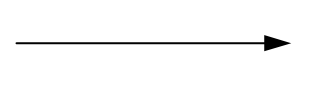
\includegraphics[width=\textwidth]{img/bpmn-sequence.png}
        \caption{Evento}
    \end{subfigure}
    \hfill
    \begin{subfigure}[b]{0.3\textwidth}
        \centering
        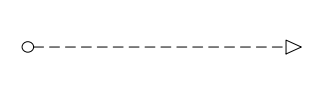
\includegraphics[width=\textwidth]{img/bpmn-message.png}
        \caption{Actividad}
    \end{subfigure}
    \hfill
    \begin{subfigure}[b]{0.3\textwidth}
        \centering
        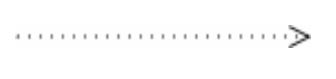
\includegraphics[width=\textwidth]{img/bpmn-association.png}
        \caption{Pasarela}
    \end{subfigure}
    \caption{Conectores en diagramas BPMN}
    \label{fig:bpmn-connectors}
\end{figure}

\subsection{Carriles}

Muchas metodologías de modelado de procesos utilizan el concepto de carriles como mecanismo para organizar las actividades en categorías visuales separadas con el fin de ilustrar diferentes capacidades funcionales o responsabilidades.
BPMN soporta los carriles con dos construcciones principales:

\begin{itemize}
    \item Pools
    \item Carriles
\end{itemize}

Los \textit{pools} se utilizan cuando el diagrama involucra dos entidades de negocio o participantes separados y están físicamente separados en el diagrama.
Las actividades dentro de pools separados se consideran procesos independientes. Por lo tanto, la secuencia no puede cruzar el límite de un pool.
Un flujo de mensaje se define como el mecanismo para mostrar la comunicación entre dos participantes, y, por lo tanto, debe conectarse entre dos pools.

Los \textit{carriles} están más estrechamente relacionados con las metodologías tradicionales de modelización de procesos por carriles de nado.
Los carriles se utilizan a menudo para separar las actividades asociadas a una función o rol específico de la empresa.
Una secuencia puede cruzar los límites de los carriles dentro de un pool, pero el flujo de mensajes no puede utilizarse entre los elementos de flujo de los carriles de un mismo grupo.

\begin{figure}[H]
    \centering
    \begin{subfigure}[b]{0.45\textwidth}
        \centering
        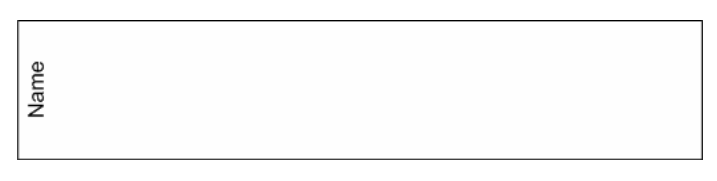
\includegraphics[width=\textwidth]{img/bpmn-pool.png}
        \caption{Pool}
    \end{subfigure}
    \hfill
    \begin{subfigure}[b]{0.45\textwidth}
        \centering
        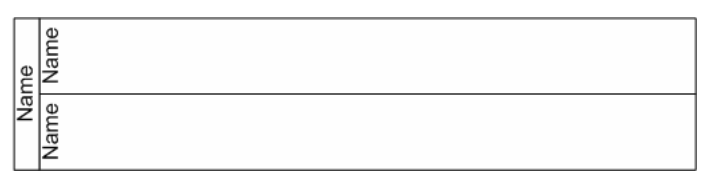
\includegraphics[width=\textwidth]{img/bpmn-lane.png}
        \caption{Carril}
    \end{subfigure}
    \caption{Carriles en diagramas BPMN}
    \label{fig:bpmn-pools}
\end{figure}

\subsection{Artefactos}

BPMN se diseñó para permitir a los modeladores y a las herramientas de modelado cierta flexibilidad a la hora de ampliar la notación básica y ofrecer la posibilidad de añadir el contexto adecuado a una situación de modelado específica.
Se puede añadir cualquier número de artefactos a un diagrama, según convenga para el contexto de los procesos de negocio que se están modelando.
La versión actual de la especificación BPMN predefine sólo tres tipos de artefactos, que son:

\begin{itemize}
    \item Documentos
    \item Agrupaciones
    \item Anotaciones
\end{itemize}

\begin{figure}[H]
    \centering
    \begin{subfigure}[b]{0.2\textwidth}
        \centering
        
\includegraphics[width=\textwidth]{img/bpmn-data.png}
        \caption{Documento}
    \end{subfigure}
    \hfill
    \begin{subfigure}[b]{0.3\textwidth}
        \centering
        
\includegraphics[width=\textwidth]{img/bpmn-group.png}
        \caption{Agrupación}
    \end{subfigure}
    \hfill
    \begin{subfigure}[b]{0.4\textwidth}
        \centering
        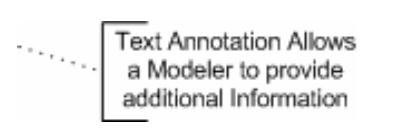
\includegraphics[width=\textwidth]{img/bpmn-note.png}
        \caption{Anotación}
    \end{subfigure}
    \caption{Artefactos en diagramas BPMN}
    \label{fig:bpmn-artifacts}
\end{figure}


\section{Análisis de la causa raíz. Cinco porqués}

El método de los cinco porqués para el análisis de la causa raíz fue desarrollado por Sakichi Toyota como parte del Sistema de Producción Toyota.
Ha sido ampliamente adoptado tanto en programas Lean como Six Sigma \cite{tarantino_smart_2022}.
A primera vista, el método de los cinco porqués parece una técnica simplista con un valor limitado, pero es eficaz y fácil de utilizar para llegar a las causas profundas de los problemas menos complejos.
Funciona porque elimina los síntomas de un problema, capa por capa, hasta llegar al "por qué" final, que es la raíz.

\subsection{Proceso}

El ejercicio de los cinco porqués mejora enormemente cuando lo aplica un equipo y hay cinco pasos básicos para llevarlo a cabo. En la Figura~\ref{fig:five-whys} se muestra una plantilla a modo de ejemplo.

\begin{itemize}
    \item Reunir a un equipo y desarrollar el planteamiento del problema de común acuerdo. Una vez hecho esto, se decide si se necesitan más personas para resolver el problema.
    \item Se pregunta el primer "por qué" al equipo: ¿por qué se produce tal o cual problema? Probablemente habrá tres o cuatro respuestas sensatas: se anotan todas en un folio o pizarra, o con fichas pegadas a la pared.
    \item Se preguntan otros cuatro "por qué" sucesivos, repitiendo el proceso para cada afirmación en el folio, la pizarra o las fichas. Coloque cada respuesta cerca de su "padre". Se realiza un seguimiento de todas las respuestas plausibles. Cuando la pregunta "¿por qué?" no aporte más información útil, se habrá identificado la causa principal. (Si es necesario, se siguen haciendo preguntas más allá de las cinco capas arbitrarias para llegar a la causa raíz).
    \item Entre la docena de respuestas a la última pregunta "¿por qué?", se buscan las causas sistémicas del problema. Se discuten con el fin de decidir la causa sistémica más probable. Después de la sesión en equipo, es recomendable un \textit{debriefing} y mostrar el producto a los demás para confirmar que ven la lógica en el análisis.
    \item Tras determinar la causa raíz más probable del problema y obtener confirmación de la lógica que subyace al análisis, se desarrollan las medidas correctivas adecuadas para eliminar la causa raíz del sistema. Las acciones pueden ser emprendidas por otros, pero la planificación y ejecución se beneficiarán de las aportaciones del equipo.
\end{itemize}

\begin{figure}
    \centering
    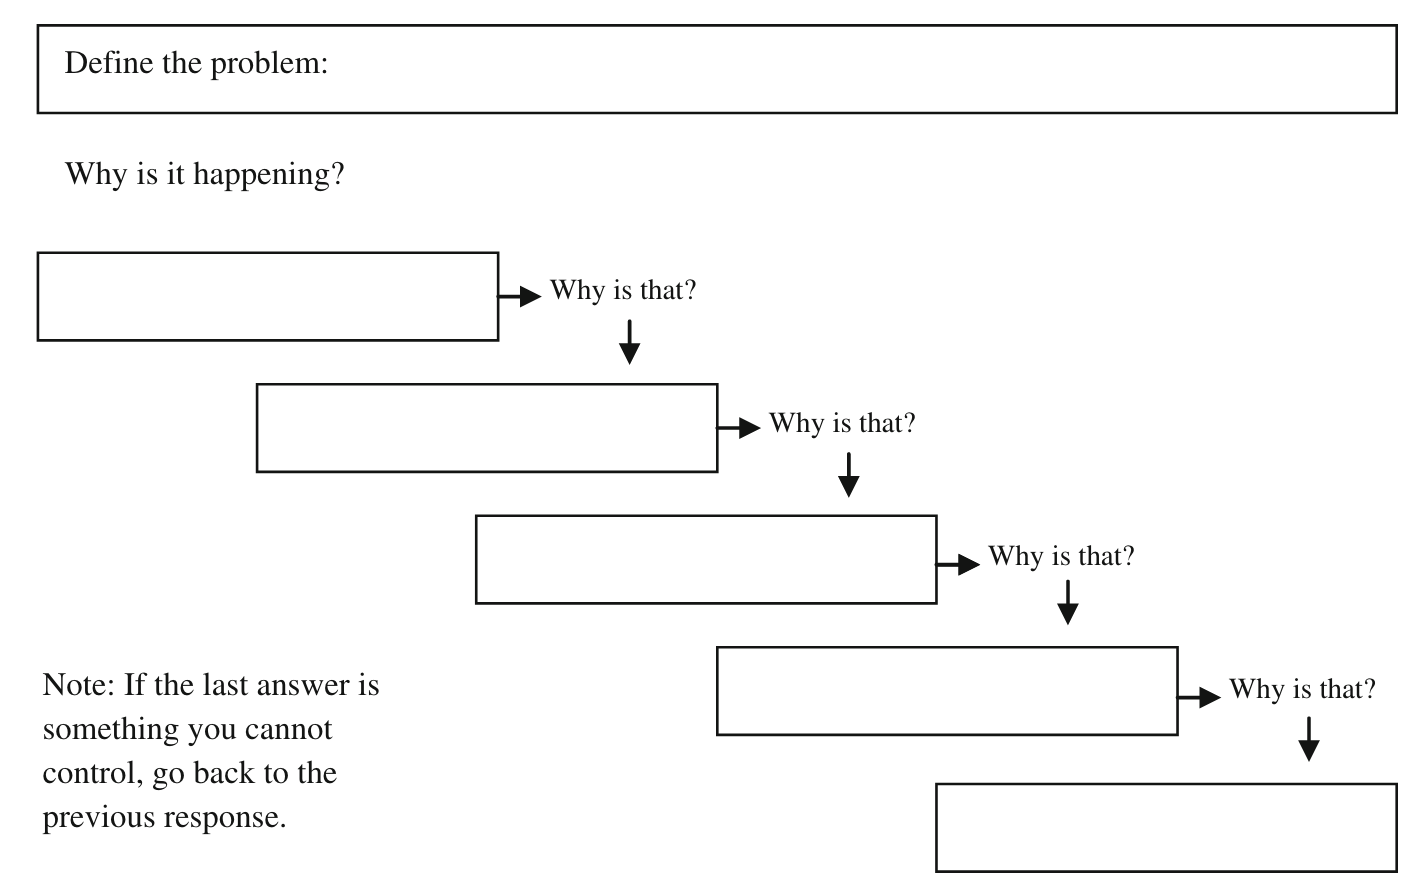
\includegraphics[width=\textwidth]{img/five-whys.png}
    \caption{Plantilla de ejemplo de los cinco porqués. Fuente: \citetitle{serrat_five_2017}}
    \label{fig:five-whys}
\end{figure}

\subsection{Precauciones}

La técnica de los cinco porqués ha sido criticada por ser una herramienta demasiado básica para analizar las causas raíz con la profundidad necesaria para garantizar que las causas se solucionan.
Entre las razones de esta crítica se incluyen:

\begin{itemize}
    \item La tendencia de los investigadores a detenerse en los síntomas y no proceder a las causas profundas de nivel inferior.
    \item La incapacidad de los investigadores para ir más allá de la información y los conocimientos actuales.
    \item Falta de facilitación y apoyo para ayudar a los investigadores a formular las preguntas adecuadas.
    \item La baja tasa de repetición de los resultados: se sabe que diferentes equipos que utilizan la técnica de los cinco porqués llegan a diferentes causas para el mismo problema.
\end{itemize}

Es evidente que la técnica de los cinco porqués se resentirá si se aplica únicamente por deducción \cite{serrat_five_2017}.
El proceso articulado anteriormente fomenta la verificación sobre el terreno de las respuestas a la pregunta "por qué" actual antes de pasar a la siguiente, y debería ayudar a evitar estos problemas.

\chapter{Desarrollo del proyecto}
En este capítulo se explica se desarrollan en detalle todos los procesos que se llevan a cabo en la sección administrativa del centro.

\section{Distribución de la plantilla}

El equipo administrativo del centro de salud está compuesto por siete miembros. En la Figura~\ref{fig:plano-interior} se muestra la posición de cada unos de los puestos.

\begin{itemize}
    \item Puestos de ventanilla: 1, 2, 3 y 4
    \item Puestos de interior: 5 y 6
    \item Jefe de grupo: 7
\end{itemize}

\begin{figure}
    \centering
    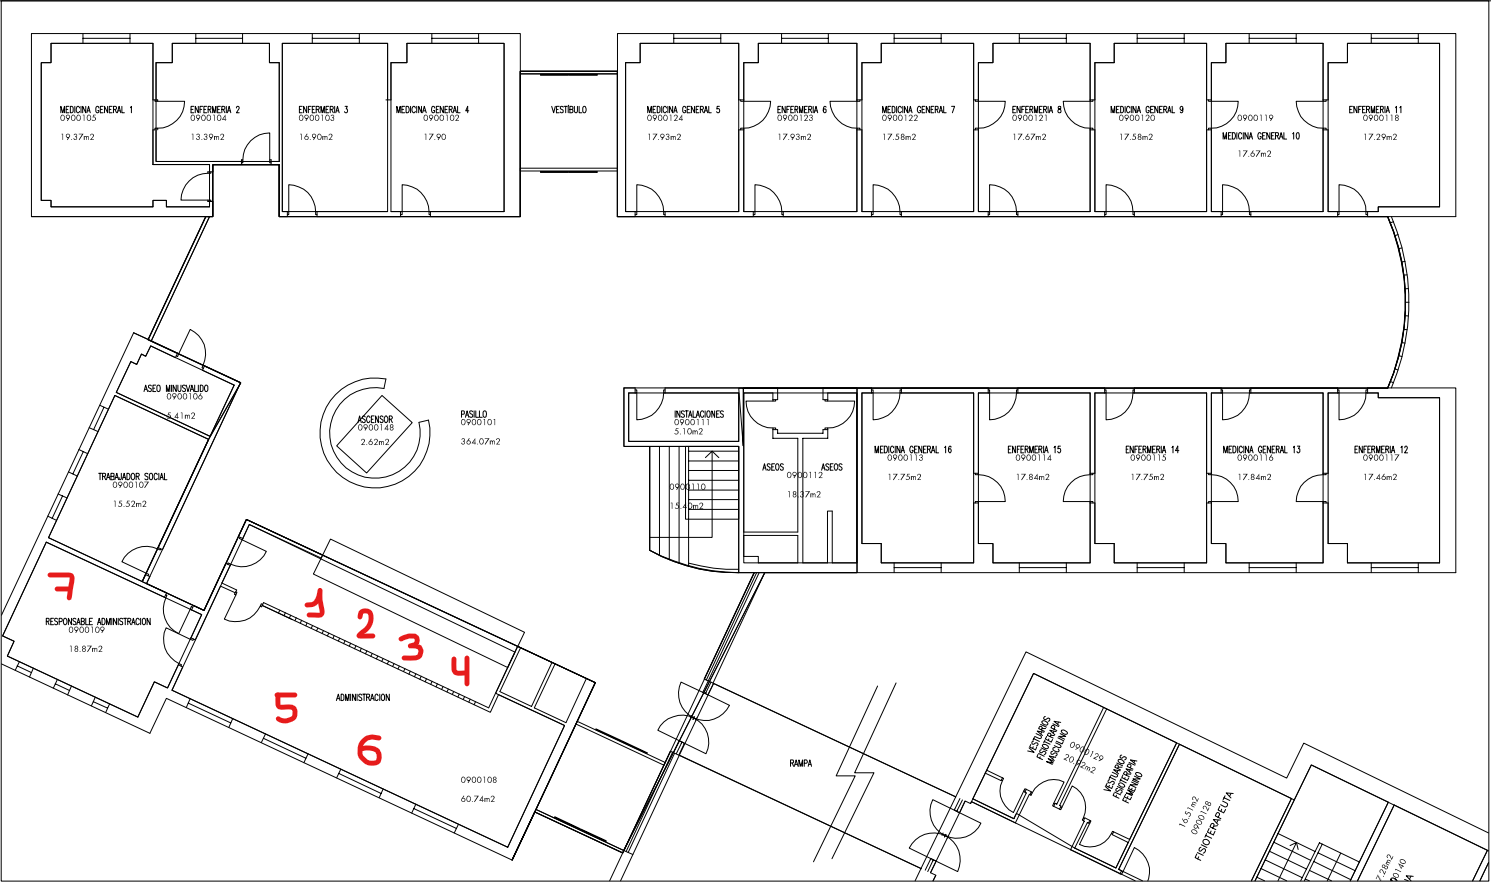
\includegraphics[width=\textwidth]{img/plano-interior.png}
    \caption{Distribución de la planta baja del centro de salud}
    \label{fig:plano-interior}
\end{figure}

\section{Procesos administrativos}

En este apartado se describen los distintos procesos que existen en la sección administrativa.
Además, se adjunto una tabla donde se especifican el estándar de tareas para cada a proceso y su diagrama BPMN correspondiente.

\begin{table}
    \centering
    \begin{tabular}{p{8cm}lll}
        \toprule
        Tarea                                                & Proceso          & Programa & Carga \\
        \midrule
        Atender teléfono rojo                                & General          & Ninguno  & 10\%  \\
        Atender teléfono urgencias local                     & General          & Ninguno  & 10\%  \\
        Diseñar carteles                                     & General          & Ninguno  & 10\%  \\
        Notificación de EDOs                                 & General          & Medora   & 10\%  \\
        Informes estadísticos                                & General          & Ninguno  & 10\%  \\
        Petición y remisión de historias clínicas.           & General          & Ninguno  & 10\%  \\
        Transferir paciente entre facultativos               & General          & Medora   & 10\%  \\
        Gestionar citas interhospitalarias                   & Gestión de citas & Hcis     & 10\%  \\
        Reubicar paciente por ausencia de médico             & Gestión de citas & Medora   & 30\%  \\
        Solicitud de citas previa en lote para   residencias & Gestión de citas & Medora   & 10\%  \\
        Recepción de solicitudes de permiso                  & Permisos         & Ninguno  & 10\%  \\
        Recepción de solicitudes de permisos aprobadas       & Permisos         & Ninguno  & 50\%  \\
        Envío de reclamaciones al servicio correspondiente   & Reclamaciones    & Ninguno  & 10\%  \\
        Dar de alta trabajadores en Medora                   & General          & Medora   & 10\%  \\
        Impresión  de pegatinas para analíticas              & Gestión de citas & Medora   & 100\% \\
        \bottomrule
    \end{tabular}
    \caption{Lista de tareas estandarizadas para el puesto de interior}
    \label{tab:gestion-citas}
\end{table}

\subsection{Gestión de citas previas}

Un paciente puede solicitar una cita con un profesional sanitario de atención primaria por dos vías: en el propio centro de salud o a través de la aplicación de SACYL Conecta.
Si el usuario decide solicitar cita previa vía online la realización de la tarea es diferida, no tiene por qué realizarse en el momento.
De esta forma, al final de la jornada o cuando el trabajo lo crea oportuno, se revisan las peticiones de citas y se tramitan en el programa Medora.
Por el contrario, si el usuario acude al centro de salud, la cita se programa en el momento, entregando un justificante en papel.
Todas las citas se programan a través de \textit{Medora} aunque hay algunas diferencias dependiendo del profesional al que vaya destinado.

En los diagramas expuestos en las Figuras~\ref{fig:proceso-consultas} y \ref{fig:proceso-pruebas} se muestra el flujo administrativo desde que el usuario solicita una cita hasta que la recibe.

\subsubsection{Citas médicas}

Las consultas de medicina familiar se citan en los huecos de demanda.
Sin embargo, si se trata de un parte de incapacidad temporal\footnote{Situación en la que se encuentran los trabajadores impedidos temporalmente para trabajar debido a enfermedad común o profesional y accidente, sea o no de trabajo, mientras reciban asistencia sanitaria de la Seguridad Social.} o una receta médica se citan en los huecos de consulta administrativa.
Por lo general no se cita en otros huecos a excepción de si es un aviso, que se cita en domicilio.
En este último caso siempre se debe confirmar la dirección del domicilio y el teléfono del paciente.

En el caso de que sea un aviso urgente, se llama al médico para que el paciente o el familiar le explique el estado.
El médico entonces valora si necesita atención urgente o no.

Todas las citas que se programen deben ser identificadas con la clave correspondiente.
De tal forma que no se imprimirá ninguna cita que no esté identificada: vía telefónica o por internet.

También es importante asegurarse que el paciente identificado es al que realmente se quiere dar una cita ya que puede haber confusión con pacientes de igual nombre y apellidos.
Para evitar esta situación se debe de verificar la fecha de nacimiento con el documento de identidad.

\subsubsection{Enfermería}

Por lo general, las citas de enfermería se citan a demanda.
También existe la posibilidad de poner un aviso a domicilio asegurándose siempre de confirmar la fecha de la cita, el domicilio del pacientes y su número de teléfono.
Además, se debe especificar el motivo de la consulta: curas, sondas, extracciones, etc.
En el caso de que haya que realizar una analítica se debe de fotocopiar el volante.

Los electrocardiogramas\footnote{Procedimiento simple, indoloro y rápido que registra la actividad eléctrica del corazón.} se citan con el enfermero correspondiente reservando dos huecos de la agenda ya que son pruebas más largas.

Las consultas de enfermería pediátrica se citan según el calendario del programa del niño sano, en los huecos de programada o demanda según corresponda. Si es necesario conviene hablar con los profesionales.

\subsubsection{Pediatría}

Las citas pediátricas se citan en los huecos de demanda de la agenda si es una consulta normal.

Las consultas programadas se citan en los huecos correspondientes según el calendario de revisiones del niño sano\footnote{Actuaciones preventivas y de promoción de la salud, que se llevan a cabo periódicamente con el fin de controlar que el niño se está desarrollando y creciendo de manera correcta.}, procurando que aquellas que corresponden a pediatra y a enfermera coincidan en el mismo día.

Los huecos RN se deben de asignar a las revisiones de neonatos entre los cinco y siete días de vida.

Las urgencias pediátricas se citan en los huecos de enfermería forzando, si es necesario, la cita. Si la enfermera que corresponde al paciente no se encuentra disponible, se asigna la cita con otra enfermera.
En el caso de niños desplazados o transeúntes que deban ser citados de urgencia, se les asignará el pediatra que asuma ese día la miniguardia.

\subsubsection{Obstetricia}

Existen distintos tipos de consulta. En lo posible, hay que respetar cada tramo aunque si es necesario conviene hablar con la matrona en caso de duda.

\subsubsection{Odontología}

Las consultas de odontología se citan en la agenda correspondiente de \textit{Medora}.
El dentista suele pedir ortopantomografías\footnote{Técnica de radiografía panorámica que se sirve de rayos X para ofrecer información detallada acerca de las estructuras dentales y la anatomía oral} mediante volante. Este tipo de prueba radiológica se realiza en el Hospital Río Hortega solicitando previamente cita.
Es importante citar al paciente al día siguiente de la radiografía para que el odontólogo vea los resultados.

\subsubsection{Trabajador social}

Acude tres días a la semana: lunes, martes y miércoles.
Solo es posible citar en los huecos de demanda.

\subsubsection{Laboratorio}

Las extracciones de sangre se citan en los huecos de agenda con el mismo nombre.
En caso de que haya sido solicitada por un especialista, se debe de indicar específicamente dado que no necesita pegatina.
De la misma forma, se debe de anotar los tres últimos dígitos del número de petición en las que son solicitadas por el médico de familia.

Es importante tener en cuenta que los exudados vaginales se realizan por la matrona, no en el laboratorio.

Diariamente, se sacarán las pegatinas correspondientes al día siguiente para el laboratorio. Para ello, primero hay que imprimir el listado por orden alfabético de los apellidos desde el programa \textit{Medora}. Una vez obtenidas todas las pegatinas, es necesario comprobar que han salido todas y están correcamente impresas.

\subsubsection{Especialidades del Hospital clínico}

Ante un volante de cirugía vascular, pediátrica o torácica, se cita la consulta de la especialidad concreta en \textit{Medora}.
Se pincha en el primer hueco disponible anotando la fecha de la cita del volante y se guarda en la carpeta ``Hospital Clínico''.
Diariamente, se imprime la agenda de cada día desde \textit{Medora} y se envía vía fax junto con los volantes.
Cuando se reciben las citas, también vía fax, se espera a recibir la nota de citación.
Esta se envía al paciente haciéndolo constar previamente en la hoja que archiva en el centro.

\subsubsection{Especialidades del Hospital Río Hortega}

Para citar consultas con el programa del Hospital es imprescindible que el paciente presente la tarjeta sanitaria.
La excepción es cuando el paciente trae una hoja de citación en la que figura el número de historia clínica, el NHC.
Igualmente, es imprescindible un volante de petición de un facultativo.

Es importante comprobar que la tarjeta que entrega el paciente se corresponde con la persona que se indica en el volante.
Se vuelcan los datos de tarjeta sanitaria y se verifica la dirección del domicilio y el teléfono. De lo contrario, no se puede dar la cita.

La identificación del paciente se puede hacer, si no funciona con la tarjeta, por número de afiliación junto con los apellidos, nombre, fecha de nacimiento, documento de identidad o cualquier otro campo.

Tras la identificación, se pincha en la tarjeta sanitaria para proceder a la comprobación y volcado de todos los datos.
Si los datos no son correctos, se modifican en el programa de tarjeta sanitaria.

A continuación, en el puesto de citación, se comprueba nuevamente que la persona que aparece en pantalla es a la que realmente queremos citar.
De la misma forma, hay que tener especial cuidado a la hora de entregar la hoja de cita del paciente.

Las citas de radiología se solicitan en ventanilla y con el volante.
Se debe de indicar en el volante el número de historia clínica antes de imprimir la cita.
Este proceso se puede realizar también por vía telefónica.

Las radiografías que no se pueden hacer en el centro de salud son las columnas totales y otras más específicas que se realizan en el Centro de Especialidades Arturo Eyries.

Las ecografías se citan también en el Hospital.

Por otro lado, las citas de ginecología solo se pueden dar para los ginecólogos del propio centro de salud.
Los pacientes que deseen otro ginecólogo o en otro centro, deberán redactar un escrito y presentarlo en la sección de Atención al Paciente del Hospital Río Hortega.

\subsubsection{Citas preferentes}

Las citas preferentes que paute el profesional médico se tramitan desde el puesto de ventanilla en la consulta virtual habilitada para tal efecto.
En este caso no se imprime la hoja de cita pero la primera hoja del volante se guardará en el archivador correspondiente ``Preferentes pendientes'' por orden alfabético del puesto interior.

Las ecografías preferentes o de la unidad de mamografías, se envían por fax a Lourdes. Los nódulos tiroideos tendrán la misma consideración.

Cuando se reciban las citas, se debe hacer constar en la copia enviada, la fecha de recepción de la cita y la tramitación que se hace de ella. Si la cita es muy inmediata y no da tiempo a enviar el correo, se deja en ventanilla.
En este último caso, se llama al paciente por teléfono para comunicarle la cita y se le indica que debe pasar por ventanilla del centro de salud para recoger su citación.
Posteriormente, el documento se mueve del archivador ``Citas pendientes'' al archivador ``Resueltos''.

Cuando se reciben las citas desde la Gerencia, se comprueban que llegan todas las que se enviaron. En caso de no haber recibido alguna, se debe reclamar a la misma Gerencia.

\subsubsection{Consultas simtron}

Desde septiembre de 2016, se citan en la consulta de enfermería desde \textit{Medora}.
A excepción de los pacientes procedentes de residencias geriátricas, que se citan en el puesto interior de laboratorio.
Una vez se reciben los resultados del control de \textit{Sintrom}\footnote{Medición de la determinación del INR (Razón Normalizada Internacional) o lo que es lo mismo, saber cuánto tarda una muestra de sangre en formar un coágulo.}, se envían por fax a las distintas residencias geriátricas.

Del mismo modo, enfermería se encargará de obtener e imprimir los resultados de la prueba en el puesto interior.

En algunas ocasiones, a primera hora de la mañana una de las residencias envía vía fax la nota de Sintrom de alguno de los pacientes.
En este caso, se citará en el mismo día en la consulta de enfermería y se colocará el documento en el casillero correspondiente al enfermero.

\subsection{Tarjeta sanitaria}

En muchas ocasiones, un paciente acude al centro de salud no por necesitar atención sanitaria sino por motivos administrativos: alta en el sistema de salud, actualización de datos personales de la tarjeta o incluso un cambio de médico de familia. Para todos estos casos, existe un programa informático llamado ``Tarjeta Sanitaria'' donde se registran todos estos trámites.

\subsubsection{Paciente nuevo}

En el caso de un paciente nuevo o de un recién nacido, se añade en el programa introduciendo previamente el número del documento de identidad o el número de afiliación a la seguridad social.
A continuación, el paciente aparecerá en la base de datos de la comunidad o en la de la Seguridad Social.
Se rellenan todos los campos necesarios y se imprime el documento justificativo con el sello del centro.

\subsubsection{Modificación de datos}

Para realizar un cambio de domicilio, de número de teléfono, error en los datos de la tarjeta o la inclusión del número del documento de identidad.

Primeramente, se debe confirmar que el paciente existe en la base de datos de tarjeta sanitaria.
Si es así, se confirman o se modifican los datos que correspondan.
Si se da el caso de que el paciente esté dado de baja en el sistema, se le recupera.

El modo más rápido de identificación de un paciente es través de su documento de identidad o el número de afiliación de asistencia.
También cabe la posibilidad de que sea un alta nueva o un cambio de domicilio, de Gerencia o incluso la emisión de una tarjeta de desplazado.

Los mayores de catorce años, además de la inclusión del documento de identidad, se les asignará el médico de familia que tenga el titular. Como motivo de modificación se consignará el paso de oficio de pediatra a médico general.
Finalmente se imprime el documento y se sella.

\subsubsection{Extravío o deterioro}

Se identifica al paciente en la primera pantalla del programa.
A continuación, en la pestaña de tarjetas, se localiza y se indica si es un extravío o un deterioro.
Se imprime el documento y se sella.

\subsubsection{Desplazados}

Un paciente puede solicitar un desplazamiento con una duración máxima de tres meses que puede ser prorrogado otros tres.
Posteriormente, habría que darlo de alta en el sistema.

Primero, se identifica al paciente, se modifica y se emite la cartulina de desplazado.
Se cumplimentan todos los datos, indicando específicamente en la pantalla inicial que es un desplazamiento.
Se rellenan los datos relativos a la dirección del domicilio y el número de teléfono.

En cuanto a la asignación del médico, si viven con un familiar en el mismo domicilio, se le asignará el médico de familia.
De lo contrario, se le asigna al médico que tenga el cupo abierto.

Finalmente, se imprimr el documento justificativo y se sella.
Se debe de indicar en este momento la fecha de validez del desplazamiento.
Igualmente, se debe de comunicar al paciente que para recibir asistencia sanitaria es preciso presentar tanto la tarjeta sanitaria personal como el documento de desplazamiento.

\subsubsection{Transeúntes}

Cuando el periodo de permanencia es muy corto, inferior a un mes.
Se procede del mismo modo que los desplazamientos pero especificando en el programa que es del tipo ``Transeúnte''.

\subsection{Gestión de personal: Agendas}

En el programa \textit{Medora} se pueden buscar a los trabajadores seleccionando la categoría y especificando el nombre del profesional u otros datos.
Es importante pinchar en la pestaña de todos antes de buscar al profesional.
Se muestran todos los datos e información de la plaza del profesional además del CIAS\footnote{El Código de Identificación Autonómica Sanitaria es el número que identifica a un profesional médico.} o si es sustituto.
También es posible para dar de alta un nuevo usuario cuando no está dado de alta.

Si el profesional ya ha estado previamente en el centro de salud de Laguna de Duero, hay que recuperarle ya que aparecería de color naranja en el programa.
En la pestaña de ``Modificar'' se pasa a ``Activo'' para poder realizar la sustución u otro tipo de modificación.

Si, por el contrario, el profesinal no ha estado nunca en el centro de salud de Laguna habría que acceder a la pestaña de gestión de sustituciones y ver qué profesional falta y quién le sustituye.
Para crear una sustitución o dar de alta, se rellenan los campos de la pestaña de Gestión de Sustituciones especificando el profesional que sustituye junto con el día y la hora.

En caso de que no sea posible realizar la sustitución, se realiza una autorización siguiendo el mismo procedimiento.

Para transferir las citas del profesional ausente se bloquea la agenda de Medora del que falta indicando la fecha y la hora de las citas.

% EL proceso de realización de agendas consiste en la asignación de tareas sanitarias en la distintas franjas de tiempo de la jornada laboral. Las agendas están orientadas para el personal sanitario que pasan consulta o realizan algún tipo de prueba al paciente: médicos, enfermeras, fisioterapeutas, trabajadores sociales, etc.

\subsection{Cargos a terceros}

Por lo general, los pacientes que acuden al centro de salud tienen acceso gratuito a la cartera de servicios de Atención Primaria, sin embargo, hay ciertos casos en los que el Sistema Público de Salud no asume el coste y que por tanto se debe de cobrar al paciente.
Estos casos pueden ser:

\subsubsection{Convenios internacionales}

En este caso de debe rellenar el formulario \textit{H-111}, indicando diagnóstico, fecha de asistencia y firma del paciente.
Es muy importante presentar una fotocopia de la tarjeta sanitaria europea o un documento equivalente.

En el caso de que no se presente, se debe anotar el número de teléfono y el correo electrónico para poder contactar con el paciente desde la sección de ``Cargos a terceros'' del Hospital Universitario Rio Hortega.

También es necesario que el paciente firme la nota informativa ya que es el documento requerido para la protección de datos y el compromiso de hacerse cargo del importe del gasto.

\subsubsection{Accidentes de tráfico}

En el caso de un accidente de tráfico es necesario que el paciente rellene la ficha de asistencia sanitaria, firme la nota informativa y complete la solicitud de datos de accidente de tráfico.
Este último documento debe concordar con los datos presentes en el atestado\footnote{Documento oficial que elabora la Guardia Civil o una entidad policial local, en el que se describen los detalles de un accidente de tráfico} del accidente.

\subsubsection{Accidentes de trabajo}

En este caso tan solo es necesario rellenar la ficha de asistencia sanitaria y firmar la nota informativa.

\subsubsection{Espectáculos taurinos}

Se rellena la ficha de asistencia sanitaria junto con la firma de la nota interior.
En este caso, se debe de completar el documento ``Lesionados en espectáculos taurinos'' especificando el lugar donde se realiza el espectáculo y quién es el responsable del mismo (Ayuntamiento, asociaciones taurinas, etc).

\subsubsection{Agresiones}

En este caso tan solo es necesario rellenar la ficha de asistencia sanitaria y firmar la nota informativa.

\subsubsection{Accidentes deportivos o de caza}

Además de la ficha de asistencia sanitaria y la nota informativa, el paciente debe presentar una fotocopia de su licencia federativa junto con la información del seguro que cubre el siniestro, especificando el número de póliza y el número de siniestro.

\subsubsection{Seguros privados}

Se rellena la ficha de asistencia sanitaria junto con la firma de la nota informativa.
Se debe presentar también una copia del parte de accidente, la petición de asistencia o cualquier otro documento de acepctación del gasto que haya sido expedido por la empresa, la compañía de seguros o la mutua.
En el caso de que sea un paciente desplazado, se debe presentar la fotocopia de la tarjeta de mutualista.

\subsubsection{Particulares}

Se completa la ficha de asistencia sanitaria y se firma la nota informativa. Este último documento es muy importante ya que hace constar que el paciente se responsabiliza del importe del cargo.

\subsection{Reclamaciones}

El proceso de reclamaciones se inicia, generalmente, cuando un usuario se acerca a la ventanilla de admisión solicitando poner una reclamación.
El usuario deberá identificarse con su documento de identidad y el personal administrativo cumplimentará la hoja de reclamación a tal efecto.
Una vez tomados los datos, el administrativo entrega al usuario la correspondiente hoja de reclamaciones para que la rellene con su demanda.
Una vez entregada la hoja de vuelta por el usuario, se registra de entrada y se entrega la hoja amarilla al paciente mientras que las dos hojas restantes se quedan en administración.

Tras esta primera fase, si el objeto de la reclamación está relacionado con un trámite administrativo es el propio jefe de grupo quien contesta la reclamación. Si no es el caso, es el propio jefe de grupo quien entrega la reclamación al responsable correspondiente.

Una vez la reclamación ha sido contestada por el responsable, se envía una de las hojas a la Gerencia de Atención Primaria a través de correo físico ya que son ellos quienes se encargan de resolver formalmente la reclamación y hacérsela llegar al usuario a su domicilio.

Cuando la Gerencia de Atención Primaria resuelve una reclamación, además de enviar la resolución al usuario, se envía una copia al centro de salud donde se interpuso la demanda para que tengan constancia de que fue resuelta en tiempo y forma.
Este último paso es importante ya que hay casos en que los usuarios acuden al centro de salud preguntando por el estado de su reclamación.

\subsection{Absentismo}

La gestión de permisos retribuidos de los profesionales del centro de salud también recae en la sección administrativa.
Cuando un profesional quiere solicitar un permiso retribuido, debe completar el la la petición correspondiente.
Tras completar la petición se debe entregar al responsable, en el caso de médico se entre al coordinador del centro, para recibir la aprobación.
Si los profesionales son facultativos, por lo general, se deja la petición en el casillero habilitado del coordinador para que lo recoja en cuanto pueda.

Tras la aprobación del responsable, es el administrativo quien se encarga de ensobrar la petición y enviarla por correo físico a la Gerencia de Atención Primaria para su autorización.
Siempre se debe de adjuntar el original con las dos firmas, la del responsable y la del solicitante.
Se espera a recibir de vuelta la petición autorizada por la Gerencia y se realiza una fotocopia.
El original se entrega al profesional mientras que la fotocopia se guarda en la carpeta administrativa del mismo profesional, en la parte delantera de la ficha.

En numerosas ocasiones, debido a la lentitud del proceso provocada por el movimiento físico de papeles por correo, se da la situación de que el profesional disfruta del permiso antes, incluso, de recibir la autorización desde la Gerencia.
Más adelante, se tratará una de las soluciones propuestas para resolver este cuello de botella.

\subsection{Tareas generales}

\subsubsection{Informar al paciente}

Una de las funciones de los puestos administrativos de ventanilla es la de informar a los paciente y entregar justificantes de diversos tipos. Aunque las solicitudes en este proceso son muy diversas, en general se pueden distinguir tres tipos:

\begin{itemize}
    \item Utilización de la aplicación de SACYL Conecta
    \item Impresión del parte de baja laboral
    \item Impresión de justificante COVID
\end{itemize}

Todas estas tareas en general son sencillas y consumen poco tiempo al administrativo.

\subsubsection{Enfermedades de declaración obligatoria}

Las enfermedades de declaración obligatoria (EDO) o enfermedades de notificación obligatoria (ENO) son aquellas enfermedades que se consideran de gran importancia para la salud pública. Los médicos están obligados a notificar al centro de salud pública correspondiente por ser de especial importancia para la comunidad.

La notificación permite recoger datos estadísticos que muestren la frecuencia con la cual ocurre la enfermedad, lo cual, a su vez, ayuda a los investigadores a identificar las tendencias de la enfermedad y a rastrear sus brotes. Esto puede ayudar a controlar brotes futuros.

Todos las comunidades tienen un listado de las enfermedades de notificación obligatoria. Es responsabilidad del proveedor de atención médica, no del paciente, reportar los casos de estas enfermedades.

Para notificar la enfermedad se rellena el modelo C todos los lunes de cada semana.
Si existen hoja de declaración individual, se hace fotocopia de cada una de ellas.
Posteriormente, se registra en el programa \textit{Medora} el informe semanal y se imprimen dos copias.

% citar orden SAN/2128/2006, de 27 de diciembre

\subsubsection{Recetas con visado de inspección}

El paciente puede entregar en ventanilla recetas que necesiten un visado por inspección\footnote{Para poder dispensar determinados medicamentos y productos, la normativa farmacéutica exige el visado de las correspondientes recetas}.
Se guardan en el sobre de ``recetas-inspección'' del puesto interior y se indica al usuario que pase por el centro en ocho días naturales para recogerla.

Posteriormente se envían al a Inspección Médica por correo físico, registrando siempre la fecha de envío.
Cuando vengan selladas, se incluyen por orden alfabético de la carpeta fuelle ``Recetas visadas'' para tenerlas a mano cuando el paciente venga a recogerlas.

\subsubsection{Estadísticas de ginecología}

Diariamente, se recoge de la consulta de ginecología las estadísticas diarias.
Se contabilizan las primeras consultas de ginecología y obstetricia, junto con las revisiones de ambas.
Posteriormente, se registran los datos en el programa \textit{Medora}.

\subsubsection{Reubicación de pacientes}

Por motivos de cierre o bloqueo de las agendas de los profesionales, puede suceder que haya que reprogramar las citas ya dadas a los pacientes.
Se trata de llamar al paciente para cambiar la cita previa. Si esto sucede es importante indicar en el programa \textit{Medora} que la cita está reubicada en el campo de observaciones.

Si la cita ha sido programadas por enfermería, son ellos mismos quienes realizan la reubicación.

\subsubsection{Diseño de cartelería}

Según la programación, los viernes de cada semana, se crean los carteles correspondientes para conocer en qué consulta serán atendidos los pacientes cuyos profesionales estén ausentes.

Concretamente, se realizarán para los profesionales médicos, enfermería y pediatras.

\subsubsection{Atención telefónica}

En ocasiones, se reciben llamadas de urgencias que se deben de atender en primer término. Se transfieren al facultativo presente en el centro en el momento de la llamada.

También pueden llegar llamadas del servicio de emergencias del 112. Este tipo de llamadas no se deben de transferir al facultativo.

\section{Análisis causa raíz}

Tras modelar los procesos administrativos del centro de salud, se procedió a aplicar la técnica de los cinco porqués para averiguar las causas ráiz de los problemas presentes.
Para ello, se formó un grupo con los mismos componentes que para el modelado de procesos: un representante de cada puesto. En la Figura~\ref{fig:cinco-porques} se muestran los resultados de la dinámica.

\begin{figure}
    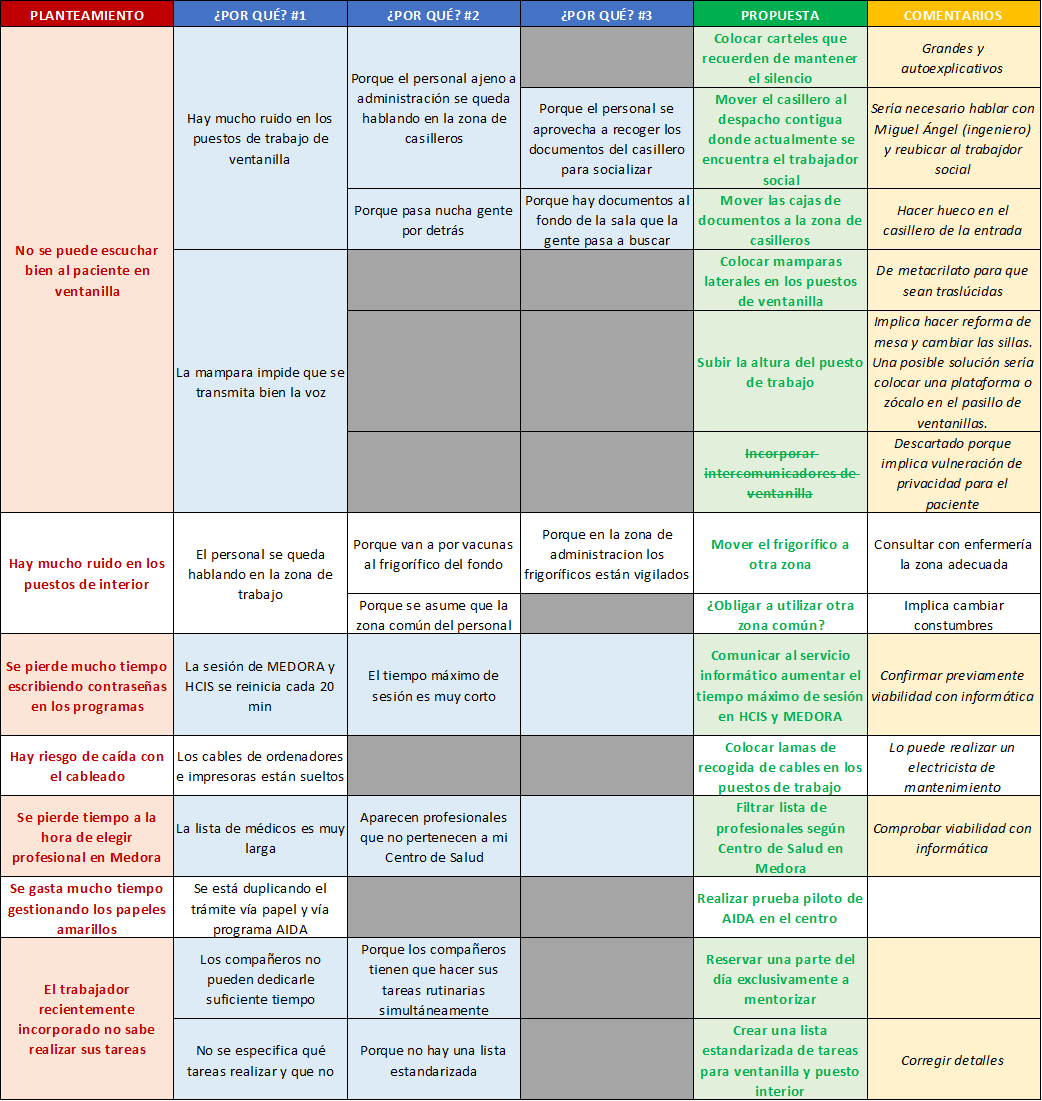
\includegraphics[width=\textwidth]{img/cinco-porques.png}
    \caption{Tabla de los cinco porqués}
    \label{fig:cinco-porques}
\end{figure}

\subsection{Comunicación complicada en ventanilla}

Los administrativos se quejan de que es difícil escuchar correctamente al pacientes al otro lado de la mampara.
Esto provoca que tengan que elevar la voz en numerosas ocasiones, lo que puede llegar a degenerar en problemas de salud.

Las causas son diversas, por un lado existe rudio ambiental en toda la zona interior de la oficina incluso estando separada del hall mediante una puerta.
Este ruido es debido al murmullo que se genera en la zona de los casilleros al concentrarse el gentío que va a recoger sus documentos.
También sucede que algunos de los documentos que no se encuentran en los casilleros, están al fondo de la sala de puestos de ventanilla lo que provoca que alguien que necesite de alguno de esos documentos se tenga que recorrer la sala pasando por detrás de los puestos.

A continuación se muestran las distintas propuestas de mejora que salieron en la reunión:

\begin{itemize}
    \item Colocar cartelería que recuerden mantener el silencio
    \item Mover el casillero al despacho contiguo
    \item Mover las cajas de documentos del fondo a los casilleros
    \item Colocar mamparas laterales en los puestos de ventanilla
    \item Subir la altura del puesto de trabajo
    \item Incorporar intercomunicadores de ventanilla
\end{itemize}

\subsection{Ruido ambiental en los puestos interiores}

En la zona interior de la sección administrativa, el personal se queja de que hay mucho ruido lo que les impide concentrarse en sus tareas laborales.
Esto es debido a que otros profesionales no administrativos lo utilizan como zona común para hablar entre ellos.
Además, muchas veces las enfermeras recorren toda la sala para recoger dosis de vacunas, ya que el frigorífico se encuentra en administración.

Algunas de las soluciones propuestas son las siguientes:

\begin{itemize}
    \item Informar al personal de que la zona de administración no es una sala de descanso
    \item Mover el frigorífico de las vacunas al sótano.
\end{itemize}

\subsection{El trabajador recién incorporado no tiene información}

Este es un problema común que existe en el ámbito sanitario debido a la alta rotación del personal.
Este problema está causado por una falta de tiempo y dedicación de los compañeros de trabajo al nuevo trabajador para enseñarle el funcionamiento de la sección administrativa. Es común que el trabajador veterano tenga que estar pendiente tanto de los usuarios de ventanilla como de las peticiones de los profesionales sanitarios. Esto hace que no se le pueda prestar la suficiente atención al trabajador nuevo y que su formación se alargue más de lo necesario.

Además, al trabajador recién incorporado no se le suele asignar tareas definidas y concretas sino que se espera de él que rinda plenamente desde el primer día asumiendo que posee todos los conocimientos necesarios. En parte, este problema surge de la ausencia de una lista de tareas estandarizadas, que es uno de los fines de este proyecto.

Entre las posibles mejoras propuestas se obtuvieron las siguientes:

\begin{itemize}
    \item Reservar una parte de la jornada exclusivamente a mentorizar al nuevo trabajador
    \item Crear una lista estandarizada de tareas para los puestos interiores y de ventanilla
\end{itemize}

\subsection{Gasto tiempo en escribir contraseñas}

Una queja común entre los administrativos es la gran cantidad de tiempo que pierden tecleando sus credenciales en los distintos programas informáticos sanitarios: Medora, HCIS o Tarjeta Sanitaria.
Esto es debido a que las sesiones de los programas son muy cortas, entre 20 y 30 minutos, lo que se traduce entre 15 y 20 veces por jornada.
En parte, esta mecánica fue diseñada para evitar que personas ajenas pudieran acceder al sistema en el caso de que el trabajador se olvidara de cerrar la sesión.

Un posible solución sería prolongar el tiempo máximo de sesión, pero no es sencillo ya que depende de servicios centrales y, en caso de realizar una modificación, habría que hacerla en todos y cada uno de los centros sanitarios de Castilla y León.

\subsection{Riesgo de caídas con el cableado}

Alrededor de las mesas de los puestos interiores se suelen acumular multitud de cables de pantallas, ordenadores o impresoras.
Se propone solicitar a mantenimiento colocar una lama que recoja todos los cables por los laterales de las mesas y así, evitar posibles caídas por tropiezo.

\subsection{Gasto de tiempo tramitando permisos}

Desde administración se quejan de que se pierde mucho tiempo tramitando los ``papeles amarillos'' ya que, aunque en los últimos años se ha implantado un programa informático para digitalizar el proceso, a día de hoy se está realizando la gestión por duplicado: vía digital y vía física.
Se plantea desde la Dirección de Gestión de Atención Primaria que el centro de salud de Laguna de Duero comience una prueba piloto con la nueva actualización del programa.
De esta forma los flujos de aprobación de los permisos retribuidos sería completamente digital.

\subsection{Analíticas no validadas}

Cuando un paciente llega a la ventanilla del centro con el volante para realizar una extracción de laboratorio, previamente el médico tiene que haber validado la analítica en el programa.
Si esto no ocurre, el administrativo tiene que buscar a un médico que valide la analítica en el momento ya que el paciente se encuentra a la espera de la prueba.
Esto genera una pérdida de tiempo considerable para el administrativo que prodría dedicarlo a otras tareas con más valor.

\chapter{Estudio económico}
En este capítulo se muestran la planificación y prespuesto económico teórico del proyecto realizado tanto a nivel de personal como de material.

\section{Fases del proyecto}

Conocer las fases del proyecto es necesario para estimar los costes económicos asociados a cada fase.
A continuación, se describen las fases en las que se ha desarollado el proyecto:

\subsection{Propuesta}

El proyecto comienza con la propuesta por parte de la Subdirección de Gestión del Área de Salud Valladolid Oeste. En esta fase se exponen los objetivos que se quieren alcanzar además de propuestas sobre la metodología a seguir.

\subsection{Preparación}

Antes de formar al grupo de trabajo del centro de salud, es necesario documentarse en la aplicación de técnicas lean y de mejora continua en entornos de oficina y sanitarios. Además, en esta fase se preparó una página web en \textit{Sharepoint} en donde ir actualizando semanalmente todo el contenido del proyecto.

\subsection{Reuniones de grupo}

Para conocer en detalle la sección administrativa del centro se organizaron reuniones semanales con un grupo pequeño de trabajadores a modo de muestra que conocieran bien su puesto de trabajo.
Se realizaron un total de seis reuniones a lo largo de dos meses.
Estas se pueden separar en dos fases, por un parte las cuatro primeras reuniones se centraron en recoger información de todas las tareas administrativas que se realizan en los puestos administrativos de cara a definir un estándar y, por otras parte, las dos últimas reuniones se centraron en obtener un listado de problemas su posterior análisis de las causas raíz.

\subsubsection{Reunión 1: Toma de contacto}

En esta primera reunión asistieron los dos subdirectores de gestión. Fue una presentación corta en la que se explicó al grupo de trabajo la necesidad de realizar una estandarización de las tareas administrativas de la sección del centro con el fin de analizar las cargas de trabajo reales. Además, se propuso de analizar mediante la técnica de los cinco porqués las causas raíz de los problemas administrativos.

\subsubsection{Reunión 2: Citas previas y tarjeta sanitaria}

Dado que la gestión de citas principales, y consecuentemente más tiempo consumen, fue el primer proceso que se trató. Se explicó con detalle los distintos tipos de citas: médico de familia, enfermera, trabajador social, ginecología, extracción y radiología. Además de explicar el proceso, se entregó una copia a modo de ejemplo de los volantes de extracciones y de radiología en los cuales el facultativo especifica qué pruebas concretas se deben de realizar al paciente.

\subsubsection{Reunión 3: Agendas, cargos a terceros, reclamaciones y absentismo}

En esta reunión se trataron los procesos de gestión de agendas, la tramitación de cargos a terceros, reclamaciones y las solicitudes de permisos retribuidos.

\subsubsection{Reunión 4: Tareas generales}

En esta última reunió sobre la estandarización se desarrollaron por parte del personal otras tareas generales que no pertenecen a ningún procesos principal.

\subsubsection{Reunión 5: Listado de problemas para los cinco porqués}

Presentación y explicación de la herramienta de los cinco porqués.
Se realizó un ``brainstorming'' para obtener todos los problemas que existen en la sección administrativas.
Posteriormente se filtraron para valorar los que más impacto tenían en el rendimiento del equipo.

\subsubsection{Reunión 6: Análisis de las causas raíz y propuestas de mejora}

En esta última reunión se fueron comentando cada uno de los problemas listados en la anterior reunión a la vez que se aplicaba la ténica de los cinco porqués.
Una vez obtenidos las causas de cada problema, se propusieron posibles soluciones a cada una de las problemáticas. Se discutió la viabilidad de cada una.

\subsection{Redacción del informe}

Finalmente, tras recoger todos los datos necesarios se procede a analizar los resultados y a redactar la memoria del trabajo.

\section{Estimación de costes}


\subsection{Costes de personal}

Los costes de personal corresponden a todas las personas implicadas en el proyecto que han dedicado parte de su jornada laboral al mismo: subdirectores y administrativos principalmente.
En la Tabla~\ref{tab:horas-trabajadas} se muestra el reparto de horas trabajadas por cada grupo de personal y por fase de proyecto.
Cabe destacar que en la columna de administrativos se ha tenido en cuenta las horas dedicadas por los cuatro trabajadores de la sección administrativa del centro de salud.

\begin{table}
    \centering
    \begin{tabular}{llll}
        \toprule
        Fases               & Ingeniero & Subdirectores & Administrativos \\
        \midrule
        Propuesta           & 8         & 1             & 0               \\
        Preparación         & 32        & 0             & 0               \\
        Reuniones de grupo  & 48        & 12            & 48              \\
        Elaboración informe & 212       & 0             & 0               \\
        \midrule
        TOTAL               & 300       & 13            & 48              \\
        \bottomrule
    \end{tabular}
    \caption{Desglose de horas dedicadas por personal y fase}
    \label{tab:horas-trabajadas}
\end{table}

Una vez obtenida la dedicación en horas se procede a calcular los costes de personal. Para ello se utilizará la tabla de retribuciones salariales de la Gerencia Regional de Salud correspondiente al año vigente, 2023, para calcular el coste por hora trabajada. Es importante, tener en cuenta que el número total de horas trabajadas por año en el Sacyl es de 1645 horas para turnos fijos diurnos.

\begin{itemize}
    \item Ingeniero: 23.13 euros/hora
    \item Subdirector de Gestión: 34.40 euros/hora
    \item Administrativo: 11.78 euros/hora
\end{itemize}

Finalmente, en la Tabla~\ref{tab:coste-horas} se muestran los costes totales de personal para todo el proyecto.

\begin{table}
    \centering
    \begin{tabular}{llll}
        \toprule
        Fases               & Ingeniero & Subdirectores & Administrativos \\
        \midrule
        Propuesta           & 185.04    & 34.40         & 0               \\
        Preparación         & 740.16    & 0             & 0               \\
        Reuniones de grupo  & 1110.24   & 277.56        & 565.44          \\
        Elaboración informe & 4093.56   & 0             & 0               \\
        \midrule
        Total               & 6939      & 447.2         & 565.44          \\
        \bottomrule
    \end{tabular}
    \caption{Coste en euros de personal por fase y posición}
    \label{tab:coste-horas}
\end{table}

\subsection{Costes de amortización}

En este apartado se han calculado los costes de las amortizaciones de los equipos utilizados en el proyecto.
Fue necesario el uso de un ordenador junto con un conjunto de periféricos.
También se incluyen las licencias de los distintos programas informáticos utilizados.

La amortización de estos equipos se ha calculado considerando una vida útil de cinco años tal y como se muestra en la Tabla~\ref{tab:coste-equipos}.

\begin{table}
    \centering
    \begin{tabular}{lll}
        \toprule
        Equipo              & Precio  & Amortización \\
        \midrule
        Ordenador HP        & 783.34  & 156.67       \\
        Licencia Windows 10 & 108.23  & 21.65        \\
        Licencia Office 365 & 127.12  & 25.42        \\
        Impresora Kyocera   & 97.23   & 19.45        \\
        \midrule
        Total               & 1115.92 & 223.19       \\
        \bottomrule
    \end{tabular}
    \caption{Amortización anual en euros de los equipos utilizados}
    \label{tab:coste-equipos}
\end{table}

\subsection{Costes indirectos}

El coste indirecto es aquel que afecta al proyecto pero que no puede imputarse a ninguna de las fases o etapas del mismo.
En la Tabla~\ref{tab:coste-indirecto} se resumen los costes indirectos del proyecto.

\begin{table}
    \centering
    \begin{tabular}{ll}
        \toprule
        Coste        & Coste \\
        \midrule
        Alquiler     & 375   \\
        Mobiliario   & 55    \\
        Electricidad & 35    \\
        Internet     & 50    \\
        Transporte   & 55    \\
        \midrule
        TOTAL        & 570   \\
        \bottomrule
    \end{tabular}
    \caption{Coste indirecto en euros del proyecto}
    \label{tab:coste-indirecto}
\end{table}

\subsection{Costes totales}

La estimación del coste total de trabajo de fin de máster se obtiene de la suma de los distintos costes totales de cada una de las partidas definidas en los apartados anteriores.
En la Tabla~\ref{tab:coste-total} se reflejan todos los costes y su peso sobre el total.

\begin{table}
    \centering
    \begin{tabular}{lll}
        \toprule
        Concepto          & Coste   & Porcentaje \\
        \midrule
        Personal          & 7951.64 & 91\%       \\
        Amortización      & 223.19  & 3\%        \\
        Costes indirectos & 570     & 6\%        \\
        \midrule
        TOTAL             & 8744.83 & 100\%      \\
        \bottomrule
    \end{tabular}
    \caption{Coste total en euros del proyecto}
    \label{tab:coste-total}
\end{table}

A estos costes habría que sumar impuestos indirectos como el IVA y el margen comercial de beneficio.

\chapter{Conlusiones}
En este último capítulo se plantean las conclusiones del proyecto y el trabajo a futuro que sería conveniente realizar en este campo.

\section{Conclusiones finales}

El presente trabajo ha tratado de aplicar técnicas de mejora continua con el fin de crear un estándar de funciones y tareas en los puestos administrativos del Centro de Salud de Laguna de Duero.

Primeramente se formó un grupo de trabajo con tres de los siete miembros del equipo: Asunción, María Ángeles y Óscar.
Con ellos se organizaron un total de seis reuniones en la que detallaron todas las tareas llevadas a cabo en los puestos administrativos. Además, en las dos últimas reuniones se comentaron los problemas más graves que afectaban a la sección.

Tras analizar todas la información recopilada se procedió a crear unas listas estándar de tareas estándar para cada proceso.
En ellas se especifica el tipo de puesto, quién demanda realizar la tarea y una estimación cualitativa del nivel de carga de trabajo que implica.
Además, para cada uno de los procesos principales se ha creado un diagrama de flujo siguiendo el estándar BPMN con la finalidad de hacer entrender mejor al lector.

Finalmente, se aplicó la herramienta de los cinco porqués para obtener las causas raíz de los problemas que más afectan al flujo de trabajo en la sección.
Analizando las causas de los distintos problemas se crearon distintas propuestas específicas para cada tema.

\section{Trabajo futuro}

Dado que este trabajo se centra principalmente en realizar la ``fotografía'' al escenario actual de la sección administrativa del centro de salud y en proponer mejoras y propuestas concretas, conviene que los siguientes trabajos continúen en esta misma línea. Concretamente, conviene que tras este trabajo se valore la viabilidad de las distintas propuestas y se implantes las que se crean más necesarias. Todo esto sin olvidar que con la implantación de mejoras se debe de realizar un seguimiento de la efectividad de cada una, por ejemplo en base a KPIs.

\appendix
\chapter{Diagramas BPMN de los procesos }

\begin{figure}
    \centering
    \begin{sideways}
        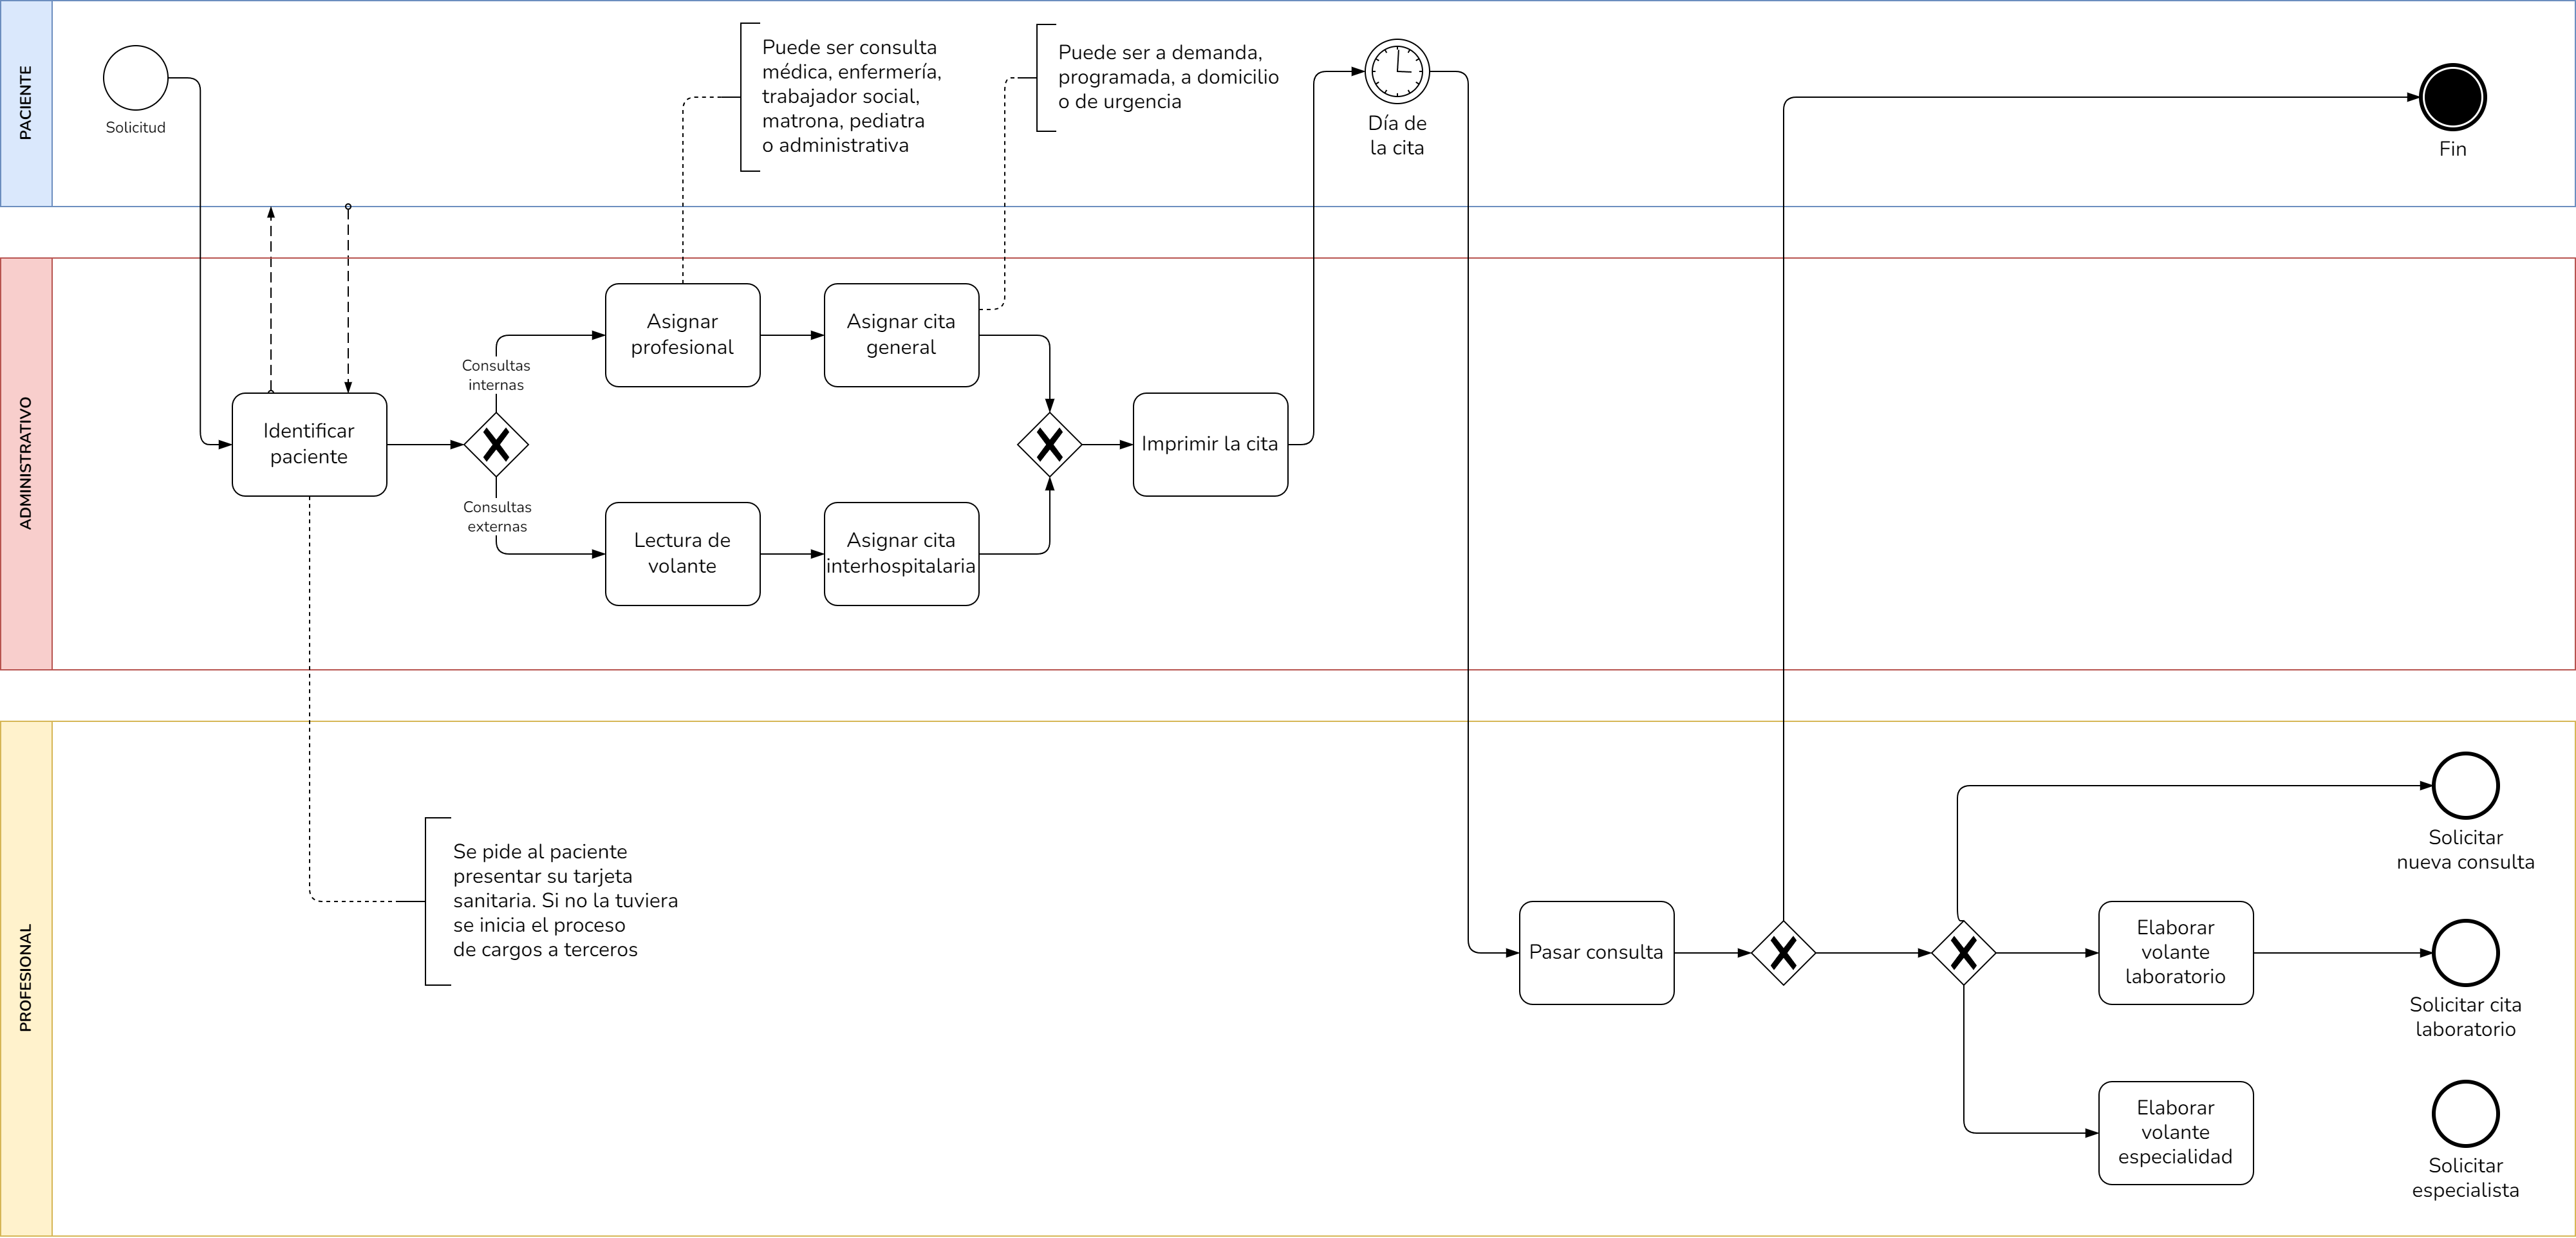
\includegraphics[width=0.95\textheight]{img/proceso-consultas.png}
    \end{sideways}
    \caption{Diagrama de proceso de consultas}
    \label{fig:proceso-consultas}
\end{figure}

\begin{figure}
    \centering
    \begin{sideways}
        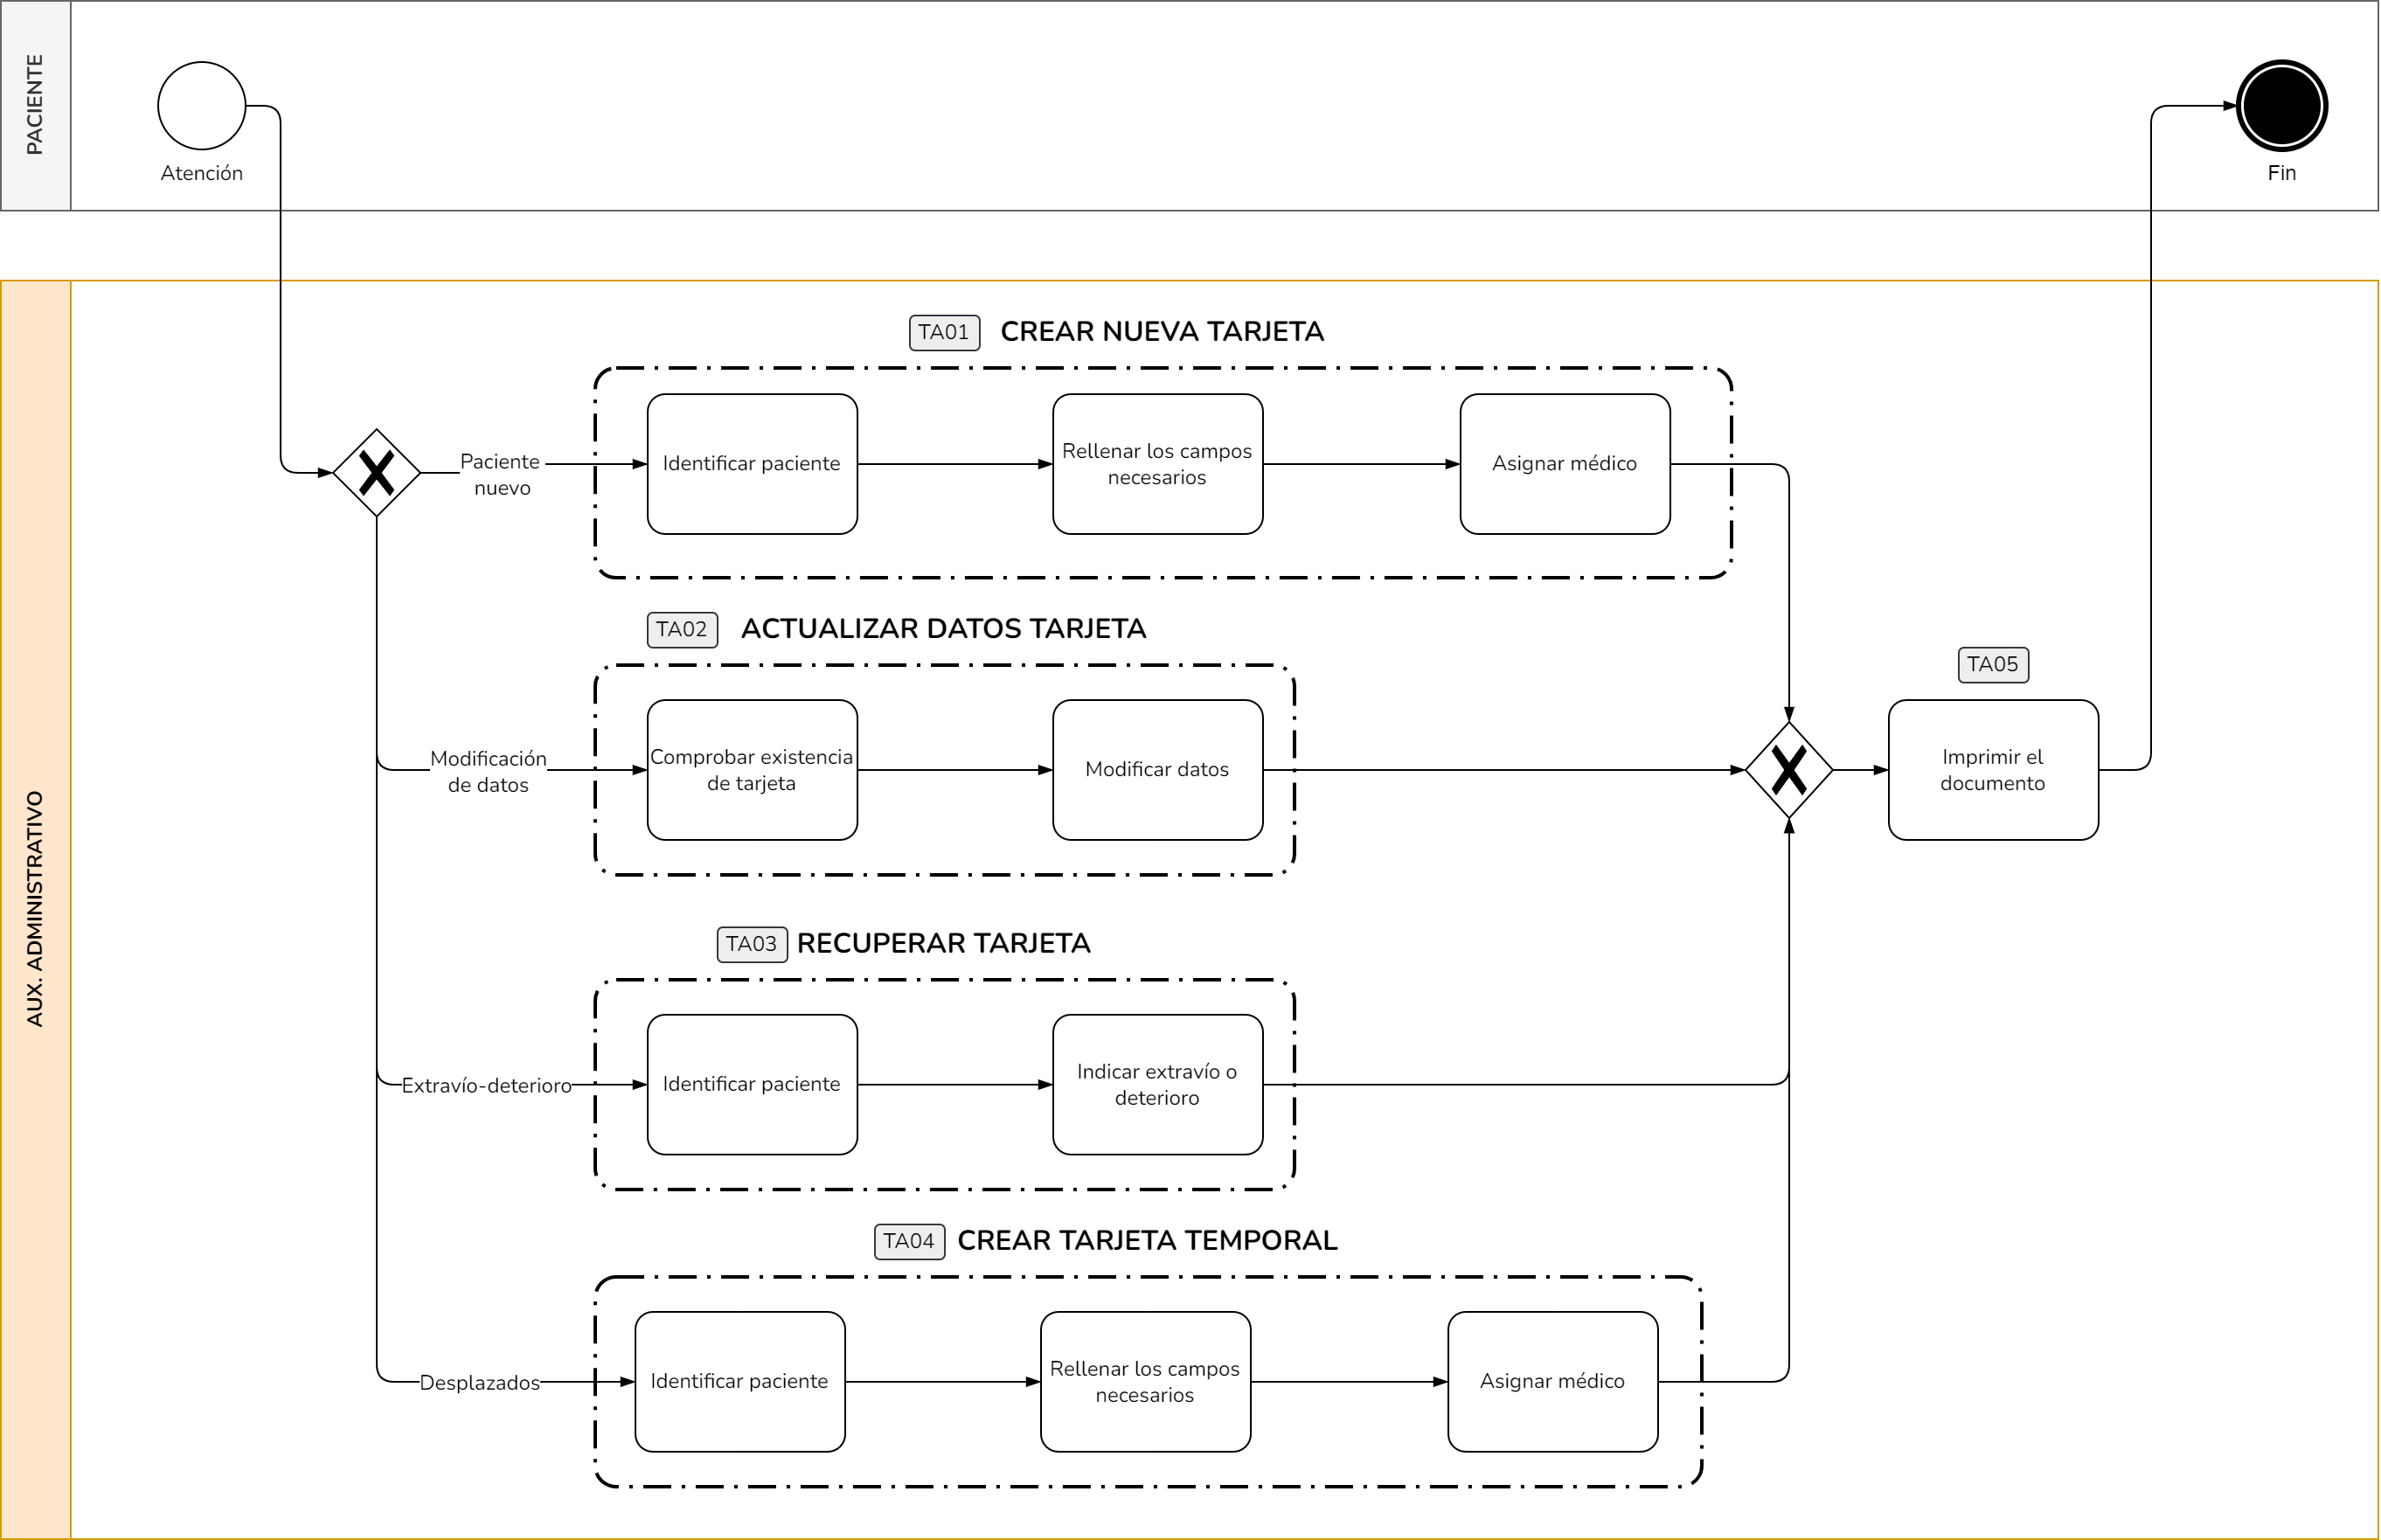
\includegraphics[width=0.95\textheight]{img/proceso-tarjeta.png}
    \end{sideways}
    \caption{Diagrama de proceso de alta o modificación de tarjeta sanitaria}
    \label{fig:proceso-tarjeta}
\end{figure}

\begin{figure}
    \centering
    \begin{sideways}
        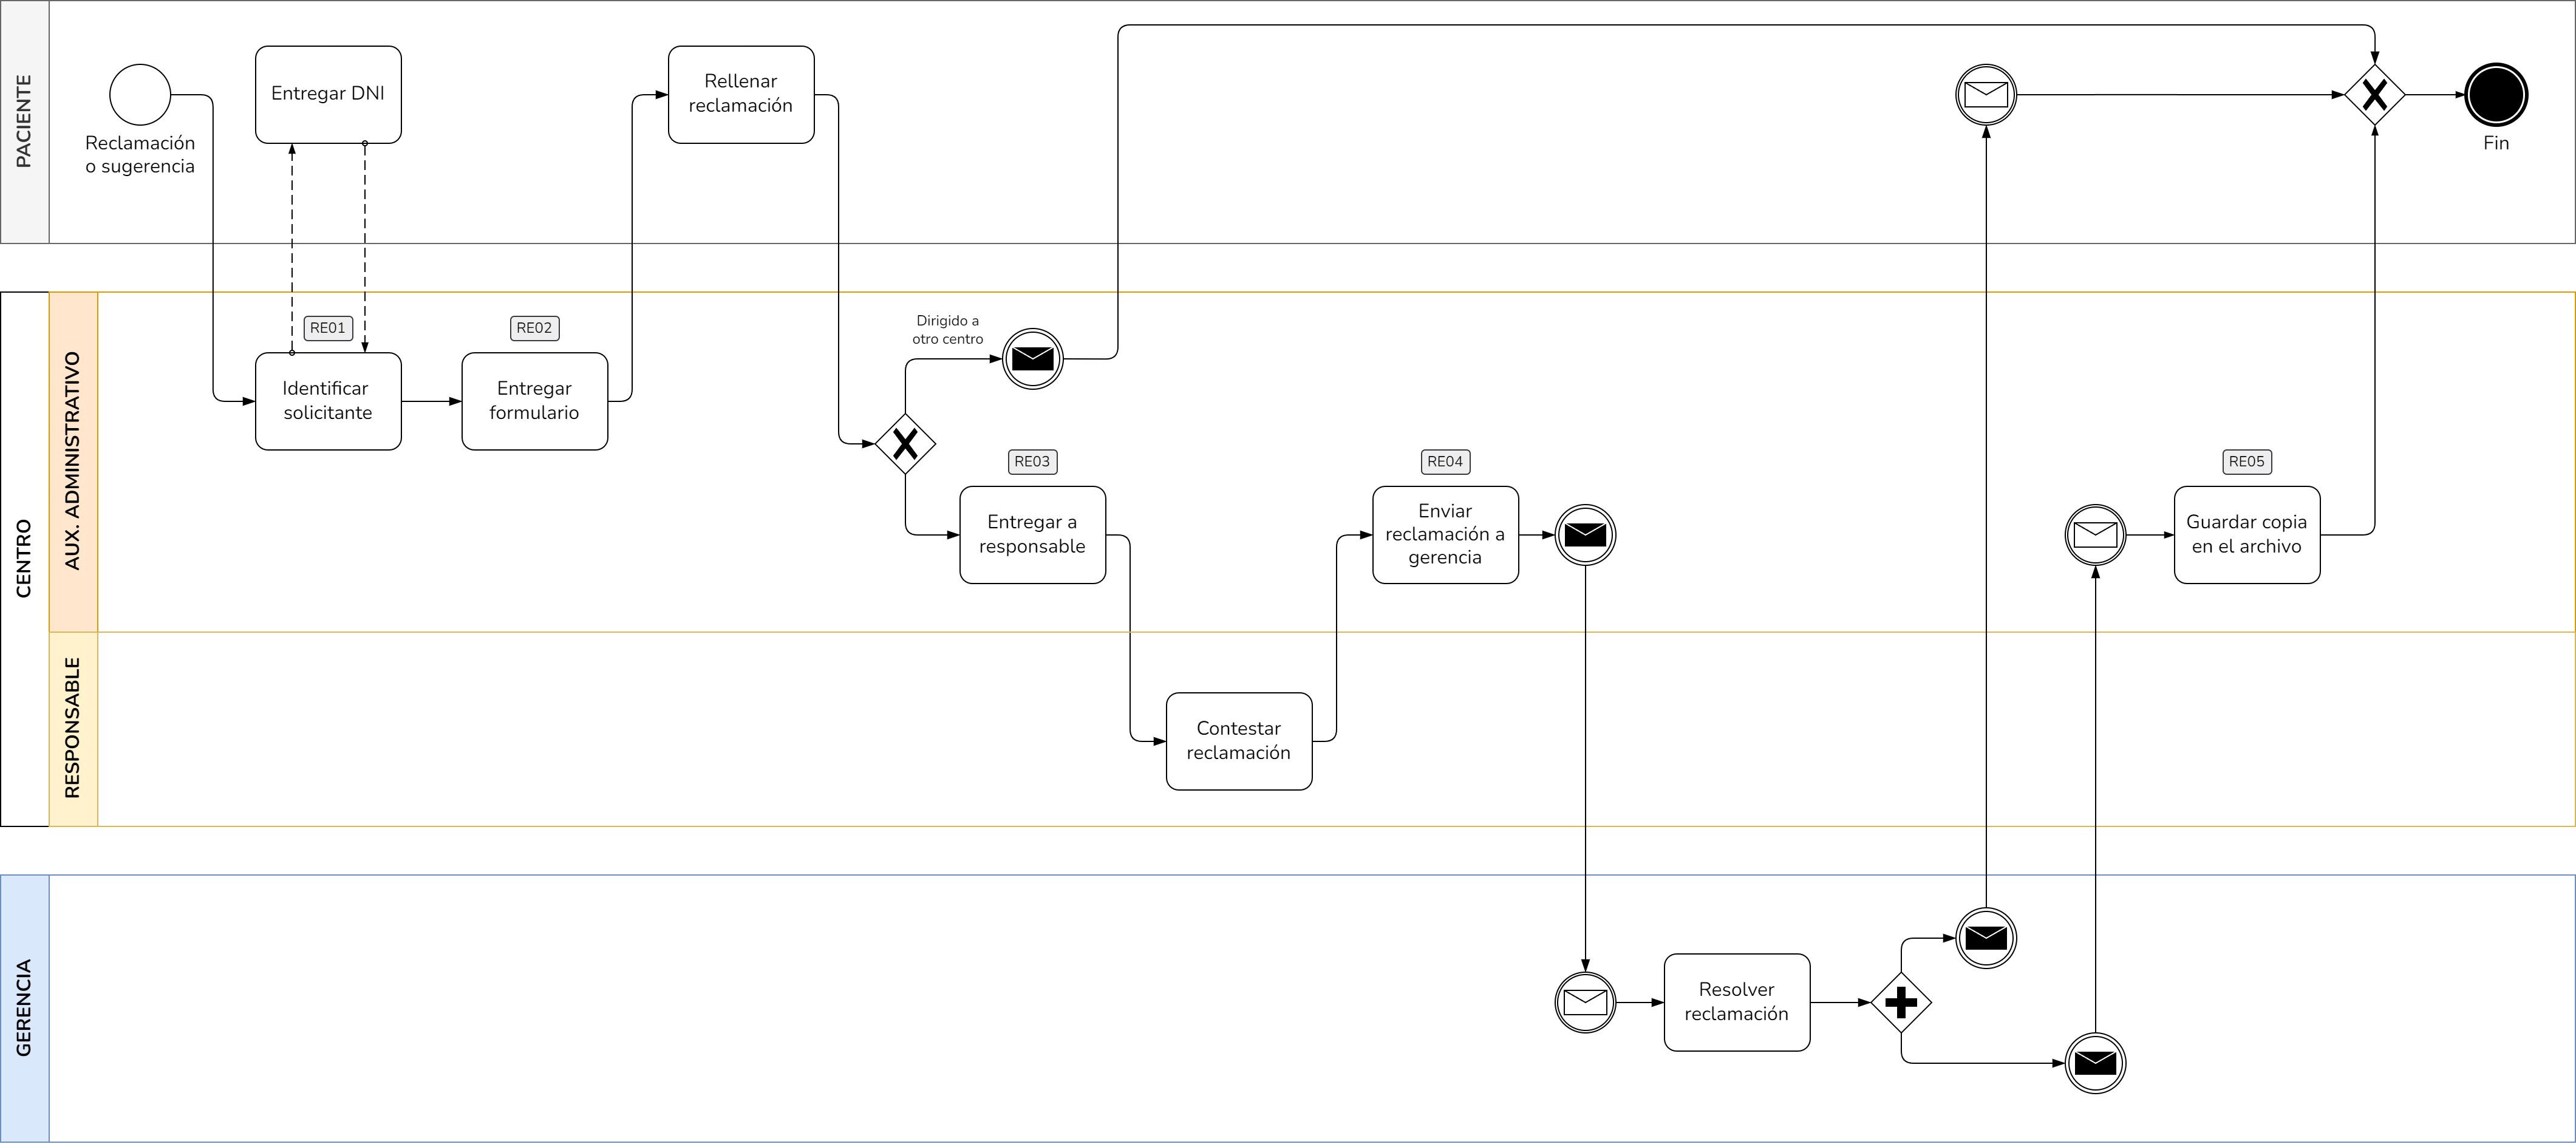
\includegraphics[width=0.95\textheight]{img/proceso-reclamaciones.png}
    \end{sideways}
    \caption{Diagrama de proceso de reclamaciones}
    \label{fig:proceso-reclamaciones}
\end{figure}

\begin{figure}
    \centering
    \begin{sideways}
        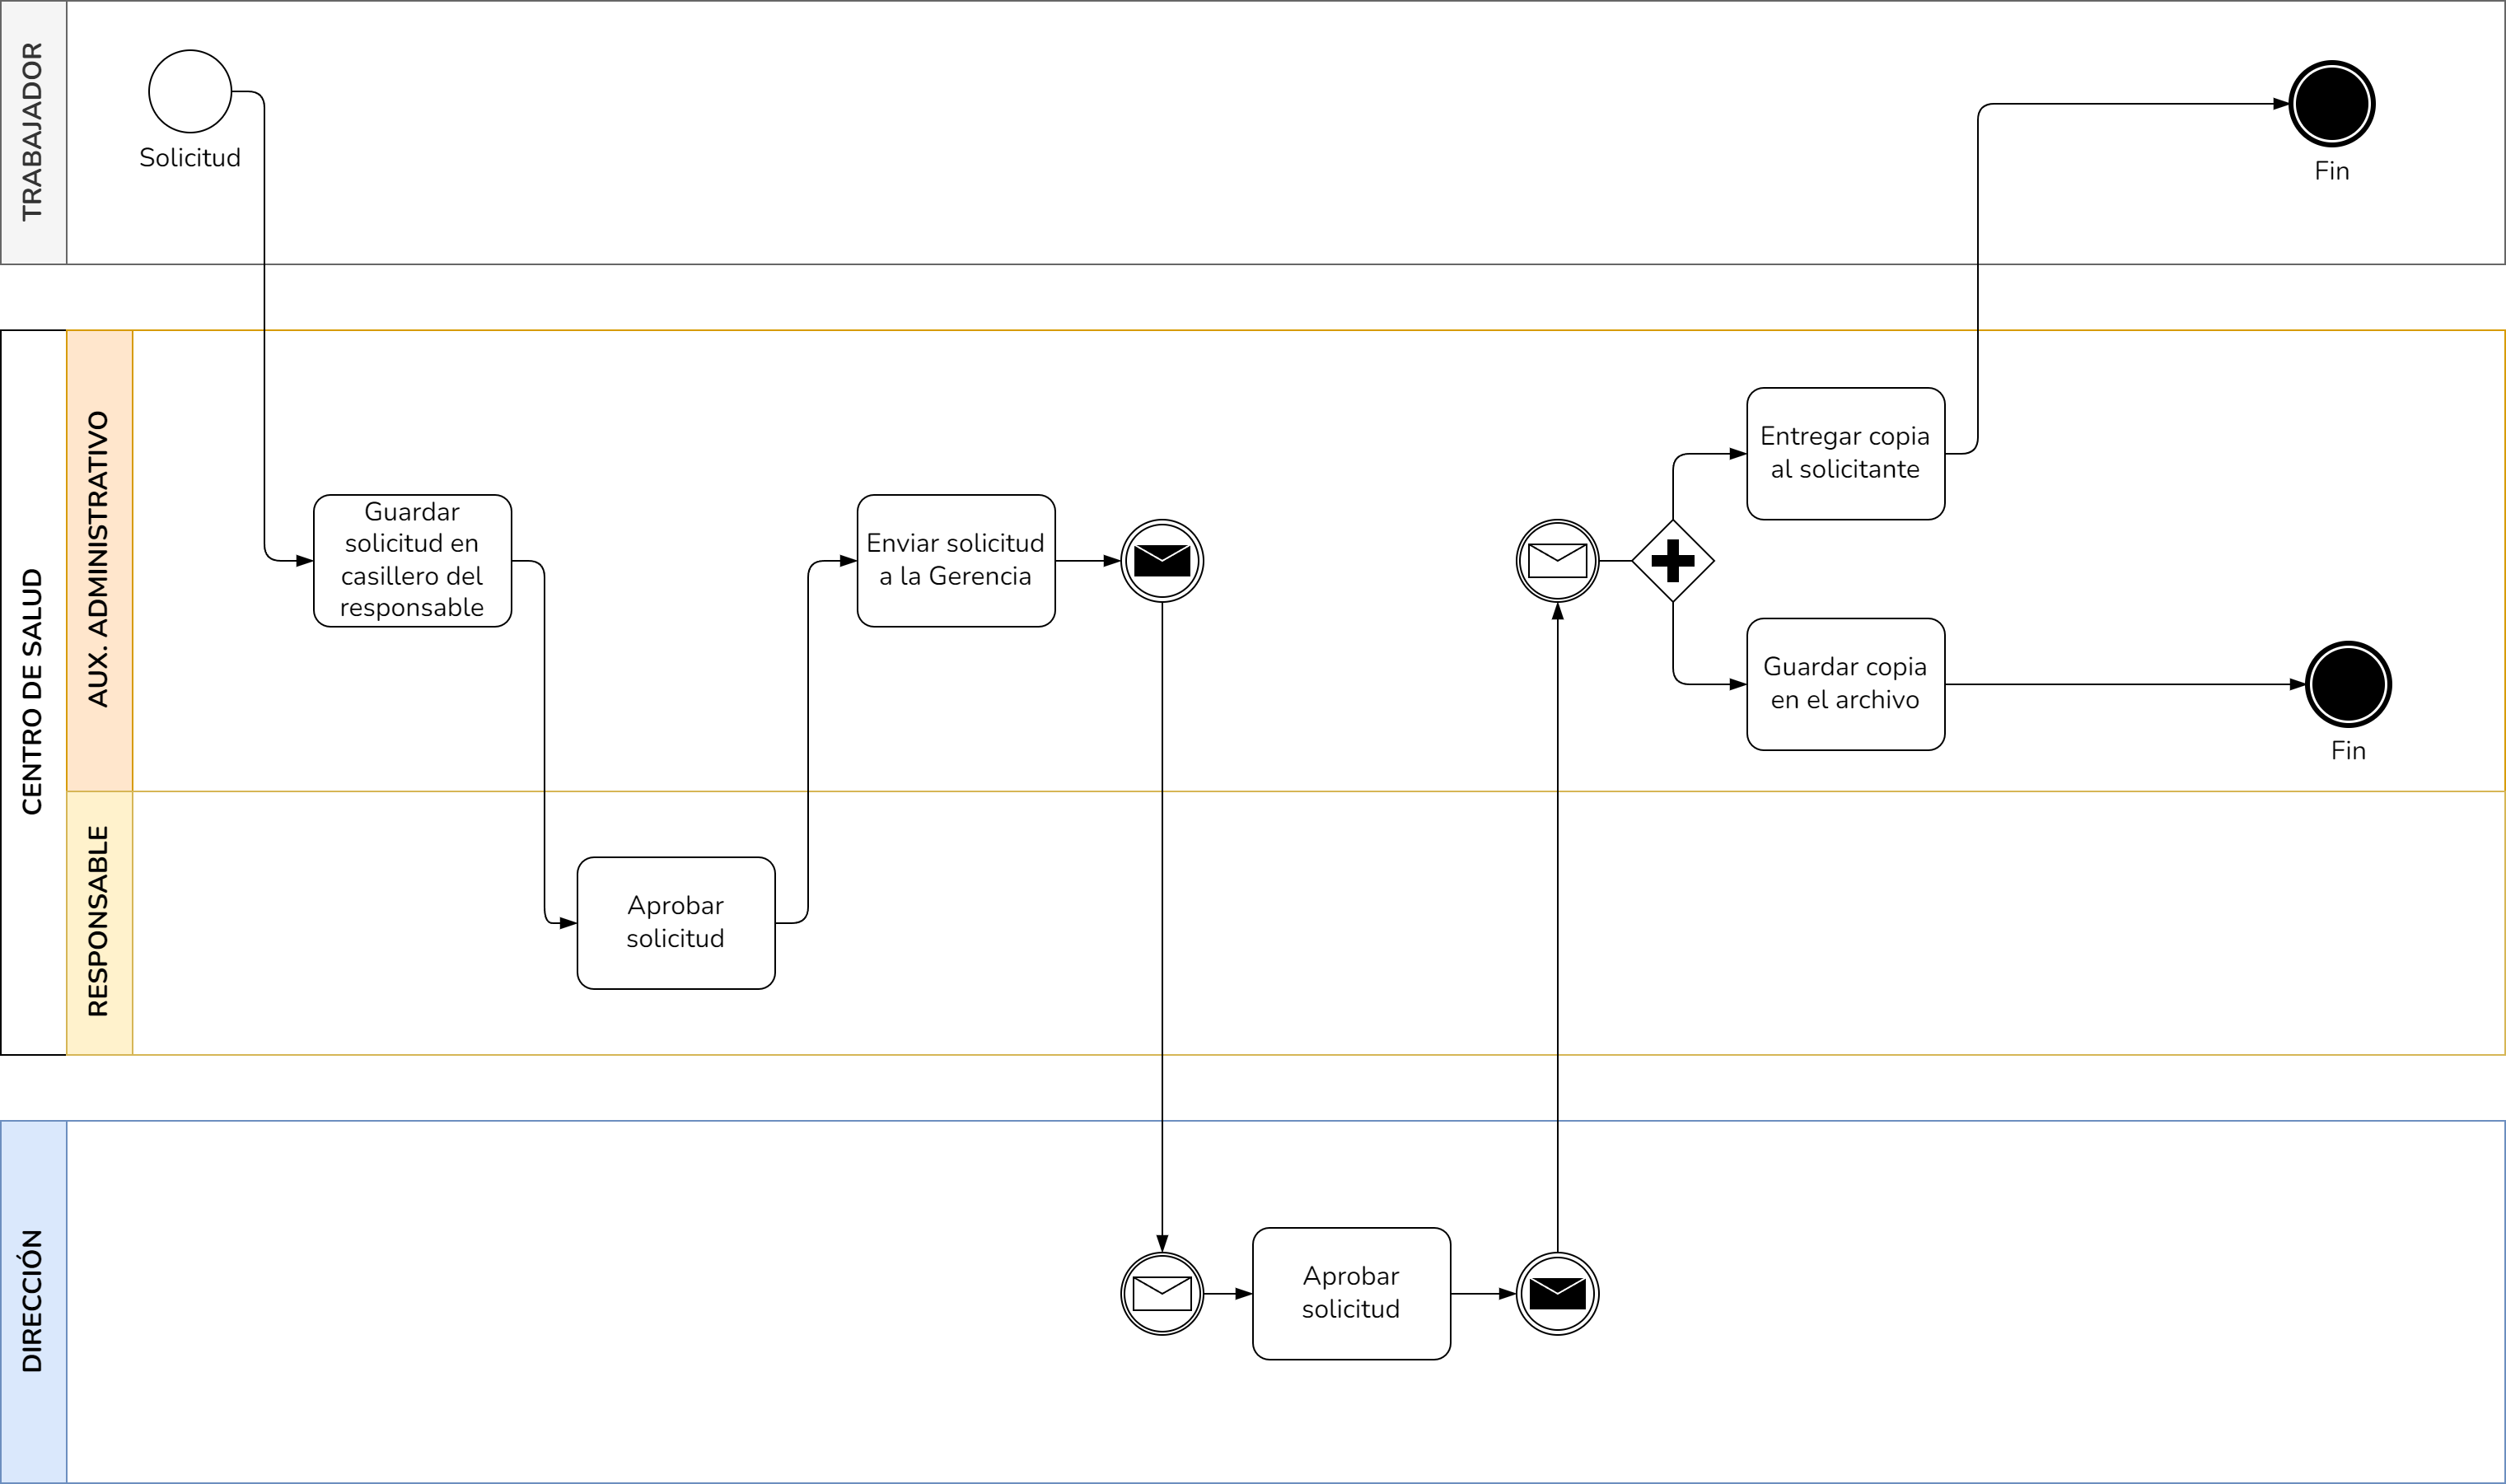
\includegraphics[width=0.95\textheight]{img/proceso-permisos.png}
    \end{sideways}
    \caption{Diagrama de proceso de permisos retribuidos}
    \label{fig:proceso-permisos}
\end{figure}

\begin{figure}
    \centering
    \begin{sideways}
        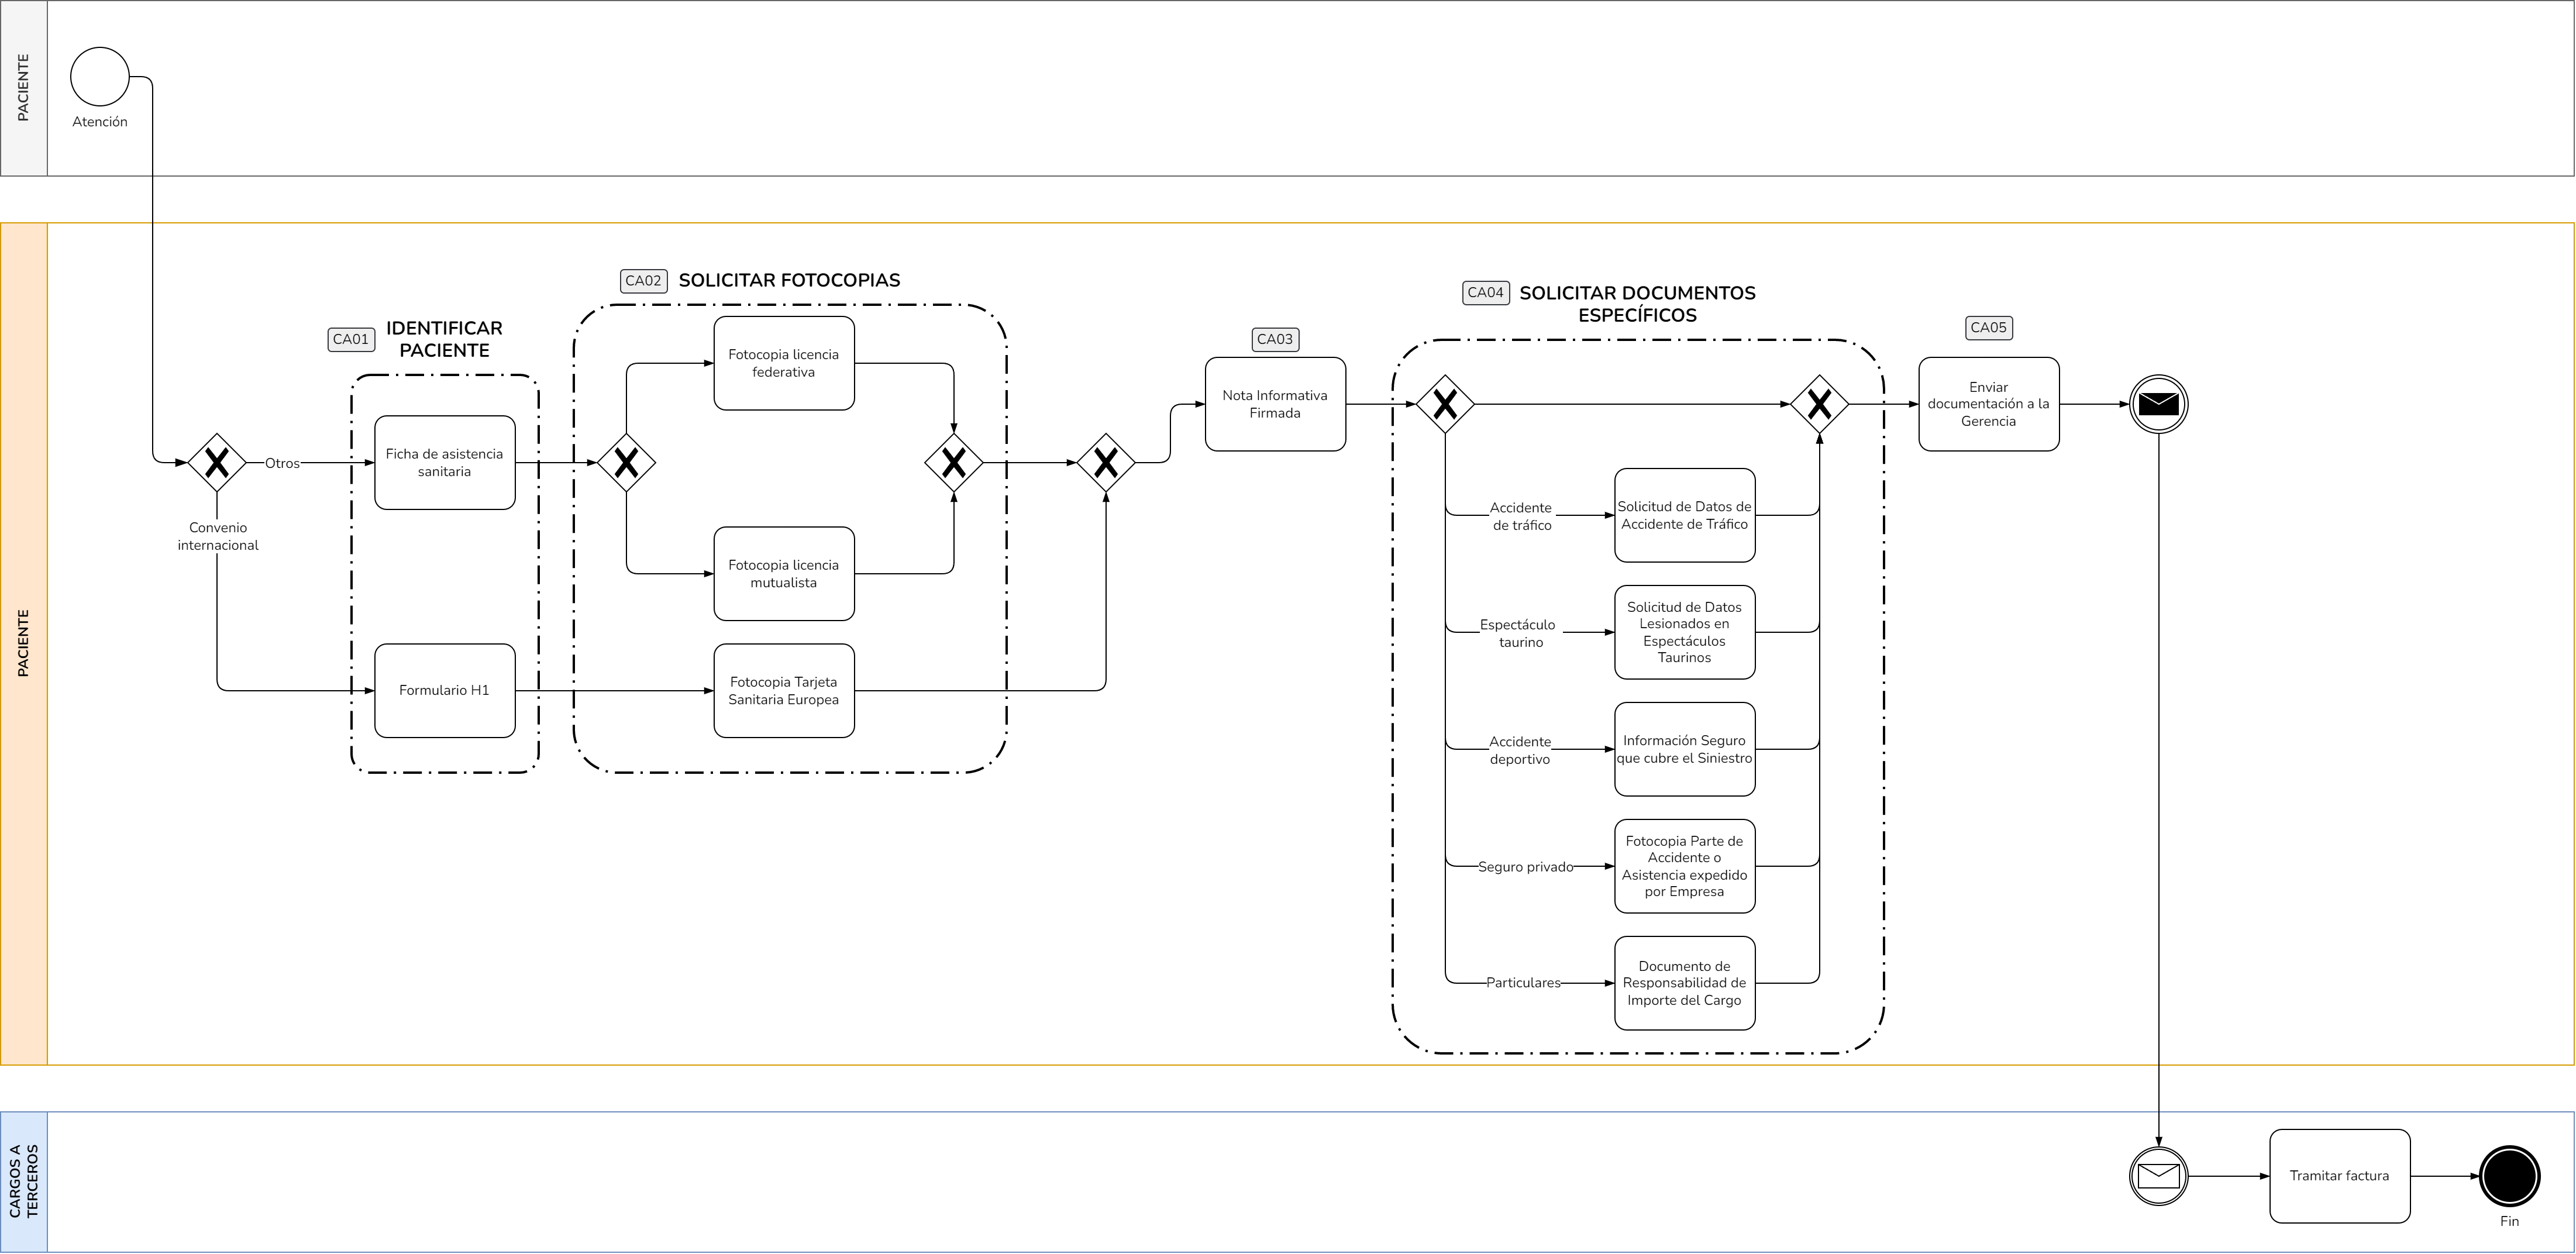
\includegraphics[width=0.95\textheight]{img/proceso-cargos.png}
    \end{sideways}
    \caption{Diagrama de proceso de cargos a terceros}
    \label{fig:proceso-cargos}
\end{figure}

\begin{figure}
    \centering
    \begin{sideways}
        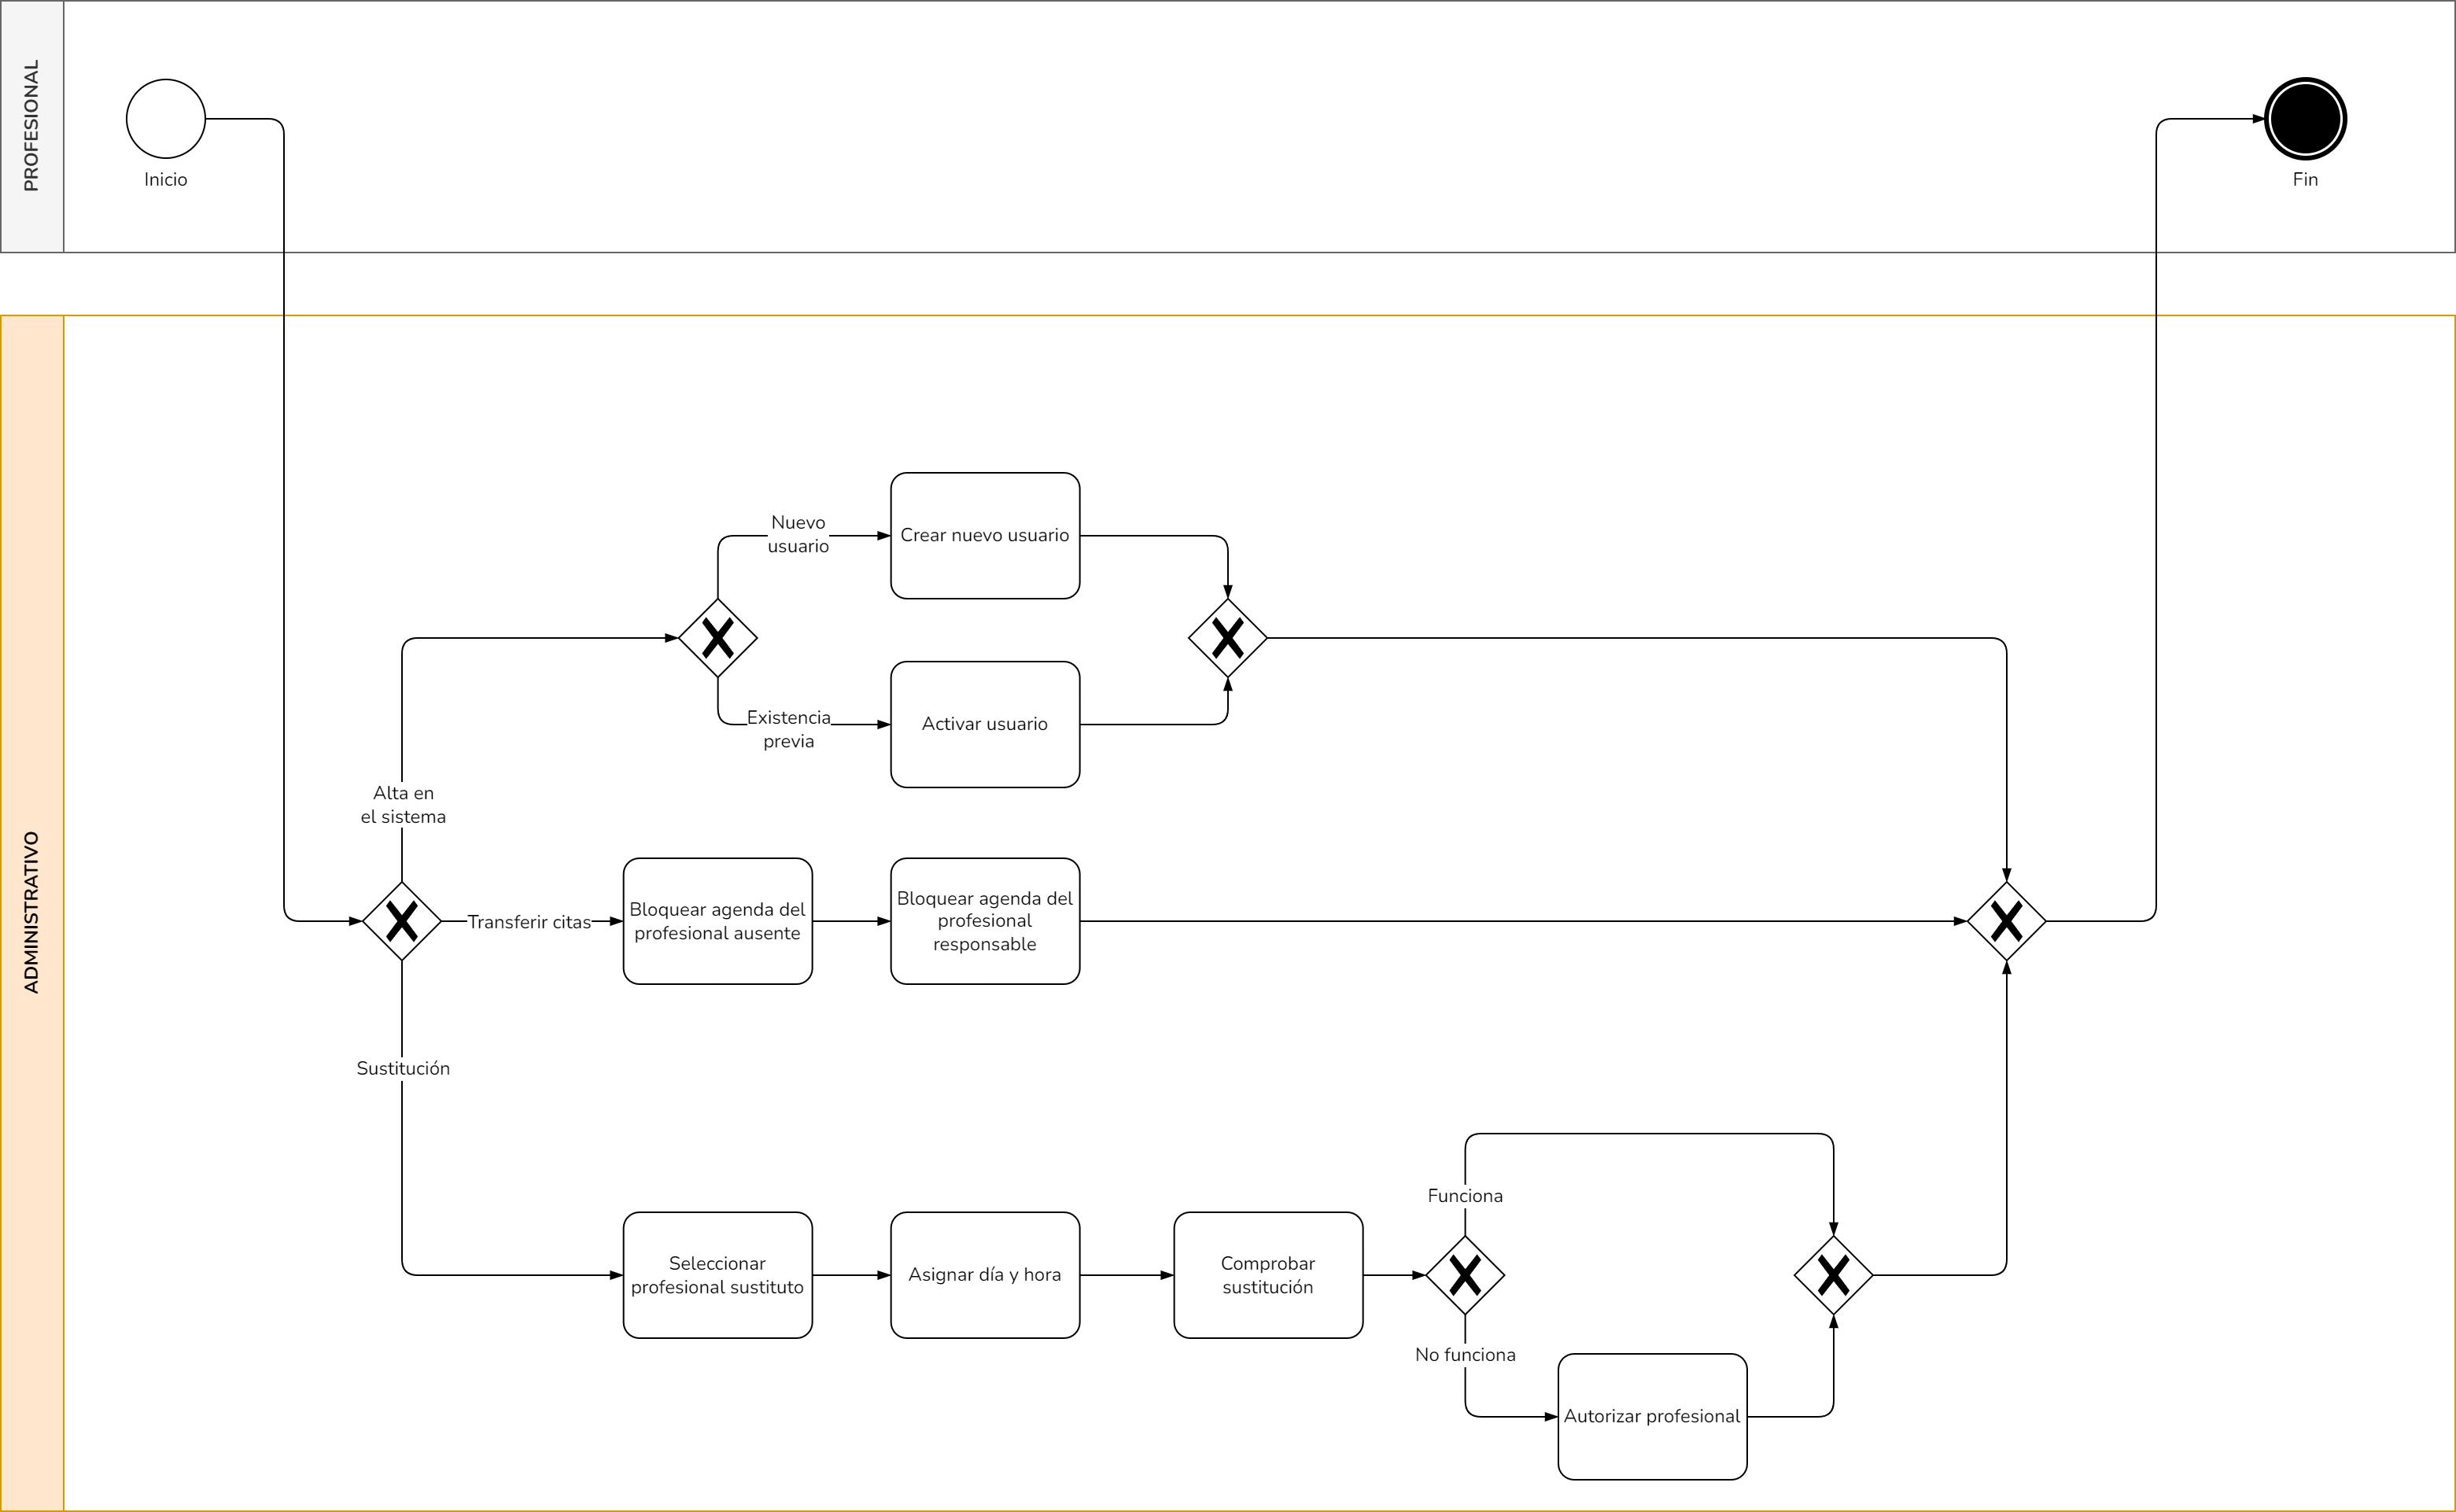
\includegraphics[width=0.95\textheight]{img/proceso-agendas.png}
    \end{sideways}
    \caption{Diagrama de proceso de gestión de agendas}
    \label{fig:proceso-agendas}
\end{figure}

\printnoidxglossaries

\printbibliography

\end{document}